\documentclass[english,bachelor]{webisthesis}

%\ThesisSetTitle{The usage of gamification in the context of human-based query obfuscation}
%\ThesisSetTitle{human-based query obfuscation with gamification}
\ThesisSetTitle{The Performance of Human Query Obfuscation - A Gamified Approach}
%\ThesisSetTitle{Human query obfuscation using gamification}
\ThesisSetKeywords{Gamification, Information Retrieval, Query, Obfuscation}

\ThesisSetAuthor{Nicola Lea Libera}
\ThesisSetStudentNumber{117073}
\ThesisSetDateOfBirth{05}{06}{1997}
\ThesisSetPlaceOfBirth{Berlin}

\ThesisSetSupervisors{Prof.\ Dr.\ Benno Stein,Matthias Hagen}

\ThesisSetSubmissionDate{29}{10}{2021}

% Packages
\usepackage{amstext}
\usepackage{amsmath}
\usepackage{amsthm}
%\usepackage[square,sort&compress,numbers]{natbib}
\usepackage{graphicx}
\usepackage{makecell}
\usepackage{wrapfig}
\usepackage[lofdepth,lotdepth]{subfig}
\usepackage{color}
\usepackage[dvipsnames]{xcolor}
\usepackage{listings}
\usepackage{mathtools}
\usepackage[makeroom]{cancel}
\usepackage{float}
\usepackage{nth}
\usepackage{textcomp}
\usepackage[protrusion=true,expansion=true]{microtype}
\usepackage{booktabs}
\usepackage{tabularx}
\usepackage{multirow}
\usepackage[all]{nowidow}
\usepackage{fancyhdr}
\usepackage{listings}
\usepackage{algorithm} 
\usepackage{algpseudocode} 
\usepackage{comment}
\usepackage{eqparbox}
\renewcommand{\algorithmiccomment}[1]{\hfill\eqparbox{COMMENT}{\# #1}}

% Settings for json example
\lstdefinelanguage{json}{
    basicstyle=\normalfont\ttfamily,
    %numbers=left,
    numberstyle=\scriptsize,
    stepnumber=1, string=[s]{"}{"},
    numbersep=8pt,
    showstringspaces=false,
    breaklines=true,
    literate=
     *{0}{{{}}}{1}
      {1}{{{}}}{1}
      {2}{{{}}}{1}
      {3}{{{}}}{1}
      {4}{{{}}}{1}
      {5}{{{}}}{1}
      {6}{{{}}}{1}
      {7}{{{}}}{1}
      {8}{{{}}}{1}
      {9}{{{}}}{1}
      {:}{{{{:}}}}{1}
      {,}{{{{,}}}}{1}
      {\{}{{{{\{}}}}{1}
      {\}}{{{{\}}}}}{1}
      {[}{{{{[}}}}{1}
      {]}{{{{]}}}}{1},
}

% Settings for footer and header
\pagestyle{fancy}
\fancyhf{}
\fancyhead[L]{\leftmark}
\fancyhead[R]{\thepage}
%\fancyfoot[C]{Gamification in Information Retrieval}

\renewcommand{\headrulewidth}{0.5pt}
%\renewcommand{\footrulewidth}{0.5pt}

% Create links in the pdf document
% Hyperref has some incompatibilities with other packages
% Some other packages must be loaded before, some after hyperref
\usehyperref

% centered tabularx column type
\newcolumntype{Y}{>{\centering\arraybackslash}X}

% add space after \forall
\let\foralltemp\forall
\renewcommand*{\forall}{\foralltemp\mkern4mu}

% obfuscation diff highlighting
\definecolor{highlightcolor}{gray}{0.87}
\newcommand{\highl}[1]{%
	\begingroup\setlength{\fboxsep}{2.5pt}%
	\colorbox{highlightcolor}{\hspace*{-2.5pt}\vphantom{My}#1\hspace*{-2.5pt}}%
	\endgroup%
}

%\DeclareGraphicsExtensions{.png,.pdf}
%\graphicspath{{./graphics/}}

% define a macro \Autoref to allow multiple references to be passed to \autoref
% thanks to Andrew <https://tex.stackexchange.com/questions/15728/multiple-references-with-autoref>
\makeatletter
\newcommand\Autoref[1]{\@first@ref#1,@}
\def\@throw@dot#1.#2@{#1}% discard everything after the dot
\def\@set@refname#1{%    % set \@refname to autoefname+s using \getrefbykeydefault
    \edef\@tmp{\getrefbykeydefault{#1}{anchor}{}}%
    \def\@refname{\@nameuse{\expandafter\@throw@dot\@tmp.@autorefname}s}%
}
\def\@first@ref#1,#2{%
  \ifx#2@\autoref{#1}\let\@nextref\@gobble% only one ref, revert to normal \autoref
  \else%
    \@set@refname{#1}%  set \@refname to autoref name
    \@refname~\ref{#1}% add autoefname and first reference
    \let\@nextref\@next@ref% push processing to \@next@ref
  \fi%
  \@nextref#2%
}
\def\@next@ref#1,#2{%
   \ifx#2@ and~\ref{#1}\let\@nextref\@gobble% at end: print and+\ref and stop
   \else, \ref{#1}% print  ,+\ref and continue
   \fi%
   \@nextref#2%
}
\makeatother

% ---- Bibliography ----------------------------------------------------

\usepackage{biblatex}
\addbibresource{literature.bib}

% custom colors
%\definecolor{dark-gray}{gray}{0.35}

% custom hyphenation rules
%\hyphenation{write-prints}

\begin{document}
\begin{frontmatter}
	\begin{abstract}
The internet is a great source to learn new things and many people use search engines to answer their information needs. However, search engines like Google save every search query in query logs which poses a risk to the privacy of users. Many different approaches exist that try to improve the privacy of searchers by distorting search profiles or hiding the user's identity. But, all of these approaches have weaknesses and need improvement. In this thesis, we research how well humans are able to obfuscate sensitive queries while still retrieving relevant web pages. Therefore, we developed City of Rebellion, a web game on the ClueWeb12 in which users have to obfuscate a given sensitive query without using any of its terms. For an obfuscated query, our game assigns points depending on the result quality of the formulated query. To help the player with their obfuscations, a list of useful search terms is provided along with a relevant document. From the data we collected in a pilot study with 72 players, we conclude that the participants were able to obfuscate sensitive queries while still retrieving relevant documents but only with the help of the given keywords.
	\end{abstract}
%	\cleardoublepage
	\tableofcontents
\end{frontmatter}

% Content
\chapter{Introduction}
Playing is part of human nature and culture \cite{huizinga}. The fact that billions of people spend several hours per week playing video games \cite{gameStatistics, numberGamers} shows how captivating games can be.
Therefore, it is no wonder, that researchers became interested in the motivational potential of video games. The idea of using "game design elements in non-game contexts" \cite{gamificationDefinition} was developed and became known as gamification. The goal of gamification is to boost the motivation and concentration of people by making (boring) tasks more game-like and therefore more enjoyable. Since the first reference of the term gamification in 2002 \cite{wirkungGamificationBuch}, the field has grown rapidly and finds usage in a wide range of applications, varying from marketing and healthcare to educational purposes \cite{ actionableGamification, gamificationExamples, gamificationHealthcareExample, gamificationHealthcareExample2}.
One of the more commonly known examples is the fitness app \textit{Zombies, Run!}, a running game that motivates users by turning every run into a mission to help people in a zombie-infested, post-apocalyptic world~ \cite{zombies}. \par
Another field of application for gamification is computer science. Especially the field of machine learning is one that has become quite important. Nowadays, machine learning is used for various applications like image or speech recognition and made the development of language assistants like Siri or Alexa possible. It is also used by big internet companies like Google or Amazon to improve their search algorithms and to provide a customized user experience. But in order to develop such intelligent systems, annotated data is needed to train the algorithms. This data must be produced by humans since computers are not able to perform this task. However, annotating or producing data is often boring and monotonous.
For this reason, computer scientists fall back on gamification to make these annotation tasks more appealing. Hence, they can collect more quality data from different people quite cost-effectively through e.g. crowdsourcing \cite{moneytaryBenefits}. \par
In this thesis, we concentrate on the appliance of gamification in relation to the field of information retrieval. Information Retrieval "is concerned with representing, searching, and manipulating large collections of electronic text and other human-language data"~\cite{informationRetrieval}. Information Retrieval systems like Google or Bing are omnipresent nowadays.
These search engines process a lot of requests from various people for a whole range of different purposes on a daily basis. While helping users to satisfy their information needs, they collect data for research purposes and to improve their algorithms to provide results specifically tailored to each individuum. Although getting customized results has its benefits, the privacy incident that occurred around AOL in 2006~\cite{aol} has shown that even anonymized data of query logs can be deanonymized when made public. The resulting danger for the privacy of users was made public by two journalists of the New York Times. In their article, Barbaro and Zeller described the case of the 62-years-old widow Thelma Arnold who could be identified through sensitive search queries like \texttt{bipolar} or \texttt{60 single men}~\cite{aol}. This is quite alarming since such search queries contain private information. These kinds of findings have motivated and still motivate computer scientists to develop algorithms that provide some kind of privacy for internet searches. Today, there exist various approaches to achieve privacy of search queries, ranging from proxy-based \cite{privateWebSearch} applications to hiding or replacing the original query by a set of dummy queries \cite{arampatzis, plausiblyDeniableSearch, trackmenot1}.\par
In this thesis, we research the ability of humans to obfuscate queries and also the strategies which they develop in the process. Furthermore, we compare the effectiveness of the obfuscated queries of humans to automatically obfuscated queries. Our findings show that humans do not perform well when it comes to hiding sensitive information needs while still retrieving relevant data.
We hope that our findings will help to improve already existing algorithms or inspire new work in the field of query obfuscation.
\chapter{Related Work}
To research the ability of humans to obfuscate queries, we developed a web game with the purpose of collecting data about possible obfuscations of sensitive search queries. First, we motivate the need for search query data protection by regarding the privacy issues of search engines and reviewing state-of-the-art techniques in the field of query obfuscation. Afterward, we illustrate why we developed a game to collect the data by explaining the effects gamification can have on the intrinsic motivation of users and their performance. And finally, we have a look at some examples for applied gamification in the context of information retrieval.\par
The internet is an enormous collection of knowledge, used by many people in their daily lives, either for work or private issues~\cite{dailyInternet}. Given the huge rise of the web~\cite{internetUsage, internetUsage2, internetWorld}, people need search engines. However, the search queries people submit to web search engines could give away private information.
For one thing, obvious information can be revealed by queries, e.g. a query \texttt{local dating} indicates that the user is single and looks for a new partner. And through profiling, data mining techniques, or classifiers even the income of users, their gender, or age can be deduced~\cite{trackmenotWeakness, classifierPrivacyAttack}. These techniques indicate that it is important that search queries stay private and can not be assigned to specific individuals. The privacy of queries becomes especially important given recent news, which report that the police have access to query logs~\cite{police}. Yet, internet companies continue to collect log files and we have seen from the example of AOL that even anonymized query logs can be deanonymized~\cite{aol}. The AOL incident is not even the only case in which the privacy of users got compromised. In 2006, Netflix published anonymized movie-rankings data from their users. With the help of very little information, researchers were able to identify some users~\cite{netflixPaper}. Another similar case happened in 1997, in which anonymized medical records could be deanonymized with the help of a publicly available voter database~\cite{privacyExamples}.\par
This shows just how much of a security problem even anonymized data can be. To tackle the problem of compromised user privacy through search engines, different approaches have been developed with the intent to hide the information need of users~\cite{arampatzis, trackmenot1, privateWebSearch, maikPaper, plausiblyDeniableSearch, knowledge, peer}. The developed algorithms can support internet users to use the Internet as usual while protecting their sensitive information needs. These algorithms are based on different ideas but follow the two basic principles of query obfuscation. They either prevent the linkability between the user's identity and a submitted query or distort user profiles. In the following, we will take a closer look at a few of them.\par
The Private Web Search \cite{privateWebSearch} plugin for Firefox is a proxy-based approach to protect the privacy of its users. It minimizes the personal data that search engines receive in every request but still returns the normal responses from queries that one would receive without the usage of this plugin. This is achieved by using an HTTP proxy to filter HTTP requests and responses before sending or receiving them through the Tor network. The filtering process removes metadata from the HTTP requests to make them indistinguishable among different users. Furthermore, the HTTP responses are filtered for JavaScript code, cookies, plugins, etc. that could reveal information about the user. Additionally, the Tor network makes it harder to distinguish users with their IP addresses and therefore to achieve query linkability.\par
Despite the elimination of personalized data, this approach has still some weaknesses. First of all, tests showed that the usage of this plugin is about 20 times slower than a normal search request~\cite{privateWebSearch} which is partly caused by the usage of Tor~\cite{torSlow}. This is a big disadvantage when it comes to usability and could potentially prevent users from installing this plugin. Second, the Tor network itself has some weaknesses that can reduce the amount of privacy of its users when exploited~\cite{torWeakness, torNew}. It is for example vulnerable to traffic analysis attacks that can deanonymize users~\cite{torInternetSurveillanceWeakness}.
Last, even though Private Web Search anonymizes its users as much as possible, it is a huge disadvantage that it does not obfuscate the search query and thus the sensitive information need of its users.\par
Other approaches like TrackMeNot~\cite{trackmenot1, trackmenot2} and the work of Arampatzis et al.~\cite{arampatzis} use cover queries to distort user profiles.
TrackMeNot is a Firefox plugin that automatically sends randomized cover queries to search engines when the browser is open. These cover queries are derived from a list of queries that functions as a seed. New cover queries are generated from an HTTP response triggered by a randomly selected query from the list. The HTTP response is parsed for suitable phrases that can serve as a new query. After the selection of a new query, the old query that started this process is deleted. This process ensures that each user has an individual list of cover queries. To simulate as well as possible the browsing behavior of its users, TrackMeNot has different strategies for scheduling the submission of the cover queries. These strategies are the usage of randomized intervals, the analysis of users' browsing behavior by their browsing history, and the utilization of so-called Query Bursts~\cite{trackmenot1}. The Query Bursts are a method that sends a series of queries to the search engine in quick succession when the user enters an actual search request. Furthermore, newer versions of TrackMeNot also prevent the identification of cover queries through technical conditions~\cite{trackmenot1}. HTTP headers, for example, can also contain user-specific data. Therefore, TrackMeNot sets the corresponding fields in the headers of the cover queries similar to the real queries. The plugin also handles active content in HTTP responses and cookies accordingly. The advantage of this idea is that the user gets the same search results that he would otherwise see without using the plugin.\par
This looks like a solid approach to achieve privacy but research has shown that TrackMeNot is not a secure system~\cite{trackmenotsogood, trackmenotWeakness}. Even standard machine-learning classifiers are able to identify user queries with an average precision of about 49\%~\cite{trackmenotWeakness}. The work of Peddinti et al.~\cite{trackmenotWeakness} also shows that the precision of identifying user queries depends on the user and ranges from 10\% up to 100\%~\cite{trackmenotWeakness}.\par
We have seen that TrackMeNot is not good at hiding the real query. This is because the plugin does not obfuscate the real query but rather submits it to the search engine. An approach that tries to achieve search privacy by actually obfuscating the real query is the work of Arampatzis et al.~\cite{arampatzis}. Instead of using simple cover queries, the actual query is replaced by a series of less private queries. Every time a user submits a search query, a bunch of new search queries derived from the original query is created. These queries are chosen by statistical means with the help of a predefined document sample. The queries are selected in a way that satisfies different privacy needs, for example, if they are suitable to obfuscate the information need while still retrieving relevant websites. After this process, the cover queries are submitted to the search engine. To present the corresponding responses to the user, the results get merged and ranked according to the original query. In addition to this algorithm, Arampatzis et al. propose to use privacy-preserving tools like Tor to prevent the linkability between the submitted queries and the user.\par
The advantage of this approach is the fact that the real query of the user is not submitted to the search engine. But the number of derived queries that have to be statistically evaluated is comparatively large which results in a higher computation effort. Furthermore, some cover queries do not obfuscate the original query very well. One example is the obfuscation of the query \texttt{gun racks} by \texttt{gun} or \texttt{gun light}~\cite{arampatzis}. This means that, without the usage of Tor or other privacy-preserving tools, third parties could draw conclusions about the actual information need of specific users. However, as we have seen before in the paragraph about the Private Web Search, Tor has its weaknesses and is slow.\par
The keyquery approach of Fr{\"o}be et al.~\cite{maikPaper} levers out an enumeration algorithm for the creation of cover queries to improve the efficiency of Arampatzis' approach by 17\% - 19\%. Still, their evaluation with increased privacy (not allowing to obfuscate gun rack with gun) showed that only 75\% of queries can be obfuscated by their algorithm. This is on par with the state-of-the-art algorithms but is far from being perfect.\par
We have seen that a broad spectrum of approaches exists to solve the challenge of privacy in conjunction with the usage of search engines. However, all these algorithms do not achieve satisfactory search privacy and still have room for improvement. That's why we want to look at the query obfuscation problem from a completely different angle.
Instead of thinking of a new algorithm to achieve privacy for users on the web, we take a look at real users. How would they obfuscate queries to protect their sensitive information need? Are they even able to do this? To collect data for this research, we used gamification and developed a little web game in which users have to obfuscate real sensitive search queries from the AOL query logs.\par
Gamification is a tool that since 2010 has gained more and more attention from various businesses and computer science sectors~\cite{wirkungGamificationBuch}. Nowadays, gamification is a market that had an estimated worth between 3 billion and 12 billion USD in 2019 and was expected to continue growing by 30\%~\cite{statistaGamificationWorth, linkedInGamificationWorth}. Even well-known companies like Audi and forums such as StackOverflow use gamification. Audi, for example, developed an e-learning game as a virtual training for their sales personal~\cite{audi} and StackOverflow uses points or "reputation" to reward active and helpful users~\cite{stackoverflow}. This is no wonder since research has shown that gamification has a high motivational potential~\cite{wirkungGamificationBuch}. Several studies indicate that the application of game design elements can have a positive effect on the intrinsic motivation \cite{intrinsicMotivation, wirkungGamificationBuch} that is "the motivation you get by inherently enjoying the task itself"~\cite{actionableGamification}. Furthermore, intrinsic motivation has a positive impact on quantitative and qualitative performance~\cite{wirkungGamificationBuch} and so does gamification~\cite{intrinsicMotivation, wirkungGamificationBuch, actionableGamification, disassembling_gamification, gamifiedSearch, gamificationMotivation}. The benefits for performance and motivation are due to the fact that the use of game elements affects the psyche by covering certain psychological needs~\cite{actionableGamification, wirkungGamificationBuch}. Apart from the boost of intrinsic motivation, the fulfillment of the psychological needs can have positive effects on the social well-being and psychological and physiological health~\cite{wirkungGamificationBuch}. To achieve this effect, there exists a wide range of game design elements.
There is a number of publications that provide an overview on several of the design elements~\cite{gameElementsListing, actionableGamification, wirkungGamificationBuch, gamificationMotivation}. Some of these publications also deal intensively with how which game design elements affect the psyche and how they can be used wisely to achieve the best motivational effect~\cite{wirkungGamificationBuch, actionableGamification, gamificationMotivation}.\par
Research has shown that the most frequently used game design elements in gamification are points, leaderboards, and badges~\cite{actionableGamification}. Depending on the sources, levels, badges, and narratives can also be included in this list~\cite{wirkungGamificationBuch, gameCrowdsourcing}.\par
Points, badges, leaderboards, and levels focus on challenge. This means that the user has to overcome problems and therefore has to develop specific skills to make progress~\cite{actionableGamification}. Points are a mean to give feedback about the user's performance. They have an enhancing effect on the performance, and the experience of competency, and some studies indicate promotion of intrinsic motivation~\cite{wirkungGamificationBuch, intrinsicMotivation}.\\
Badges and levels represent milestones and achievements of skills. These game design elements have a beneficial impact on the user's engagement and the experience of competency~\cite{wirkungGamificationBuch}. Especially levels have a positive effect on quantitative and qualitative user performance and can prolong participation~\cite{intrinsicMotivation}.\par
Leaderboards have a similar effect to levels but their effect heavily depends on their implementation. While the comparison with other users could create a sense of challenge, encouraging users to become better and outperform other users, it can also be demotivating. This negative effect could happen if someone gets stuck at the bottom of the leaderboards without a chance of rise. Therefore, developers have to take this into consideration when adding them to their games~\cite{wirkungGamificationBuch, actionableGamification, gamificationMotivation}.\\ Performance graphs also affect the perceived competence of users~\cite{wirkungGamificationBuch, gamificationMotivation}. They provide good visual feedback about the progress and achievements of each individuum. This makes people feel smarter and motivates them to improve their skills~\cite{gamificationMotivation}.\par
The other prominent game design elements narratives and avatars have a different purpose. They influence the experience of social relatedness~\cite{gamificationMotivation} and can sometimes induce task meaningfulness~\cite{wirkungGamificationBuch}.
Avatars are a mean for users to identify themselves with their virtual counterparts and users are therefore more engaged in the game. Hereby, it is important that the outlook of the avatar can be chosen. Narratives on the other hand can give meaning to an action. Furthermore, stories can act as a collective goal and support social integration \cite{wirkungGamificationBuch}. Thus, solving the tasks presented in the game becomes more important to players and improves their performance \cite{intrinsicMotivation}.\par
We have looked at examples of the effect that individual game design elements can have. However, the actual effect heavily depends on the individual player. In game theory there are different kinds of player types that respond differently to different elements, as they have different goals or motivations~\cite{wirkungGamificationBuch}. The player type Killer, for example, loves challenges and competitions in which he can outperform other players (like leaderboards). Socialisers, in contrast, prefer game elements with a social component with which they can communicate and cooperate with other players~\cite{wirkungGamificationBuch}.\par
The positive effects of some game design elements are also used by computer scientists to collect data. Especially researchers from the field of information retrieval, where a lot of data has to be collected manually, use gamification. Various games were already developed with the intent to either gather information about the search behavior of different population groups~\cite{pageFetch1, pagefetch2, fu-finder} or to get labels for websites, images, etc.~\cite{ESPlabeling, pageHunt}. In the following, we will have a further look at some examples:\par
The ESP game is a collaborative game in which two random players must work together~\cite{ESPlabeling}. These players are shown the same image for which they have to enter short descriptive strings or labels. If at some time, both of them entered the same string, they get points. The goal hereby is to collect labels for images that can be used in search engines for better retrievability. Other games to gather labeled data, in this case labels for websites, are Page Hunt, Page Race, and Page Match~\cite{pageHunt}.
In Page Hunt, players are simply shown a web page that they have to retrieve by entering search queries. If the web page is found, points are awarded. Page Race and Page Match are versions of Page Hunt but with different game dynamics. Page Race is a competitive game in which two players play against each other. Whoever retrieves the target web page first wins and gets the points. Page Match, on the other hand, is a collaborative game. Here, players must decide whether they see the same web page as their partner based on the search queries both entered. The idea of Page Hunt was also used by other researchers to gather information about the search behavior and search abilities of people. Thus, the game Page Fetch was developed, which in principle works in same way as Page Hunt but was adapted for children~\cite{pageFetch1, pagefetch2}. The objective of this version was to investigate how children perform in search tasks. Another variant of Page Hunt is Fu-Finder, a game with the goal to measure the performance of a user's querying abilities~\cite{fu-finder}.\par
The game we developed for our research is also a competitive variant of Page Hunt that possesses some additional features and game mechanics. We will have a look at the game's structure and properties in the following chapter.
\chapter{A Query Obfuscation Game}
The goal of this thesis is to research how well humans obfuscate private search queries. Therefore, we need appropriate, data about sensitive queries and possible corresponding obfuscations. Since the collection of the necessary data is a quite monotonous task, we decided to develop a web game. Using gamification makes this task more fun and potentially increases user participation. In this chapter, we give an overview of our game, its game design elements, and the development process.

\section{Game Overview}
\label{overview}
Our game, City of Rebellion, is a version of Page Hunt but with a significant difference. Just like in Page Hunt, players are shown a web page that they have to retrieve by submitting a query to a search engine. But instead of finding a search query for the web page, the associated query is already provided (see (2) in Fig~\ref{fig:game_interface}). The task of the players is to hide the sensitive information need as well as possible by obfuscating the given query while still retrieving the target document.
For the obfuscation, users are allowed to use any words or phrases, except the ones that make up the original query. Queries that contain one or more forbidden words are not accepted and the player will get an error message.
To help users to fulfill the task, a list of 10 keywords is presented (see (3) in Fig \ref{fig:game_interface}). Players will receive points if the query they submitted retrieves the target document.\par
\begin{figure}[h]
    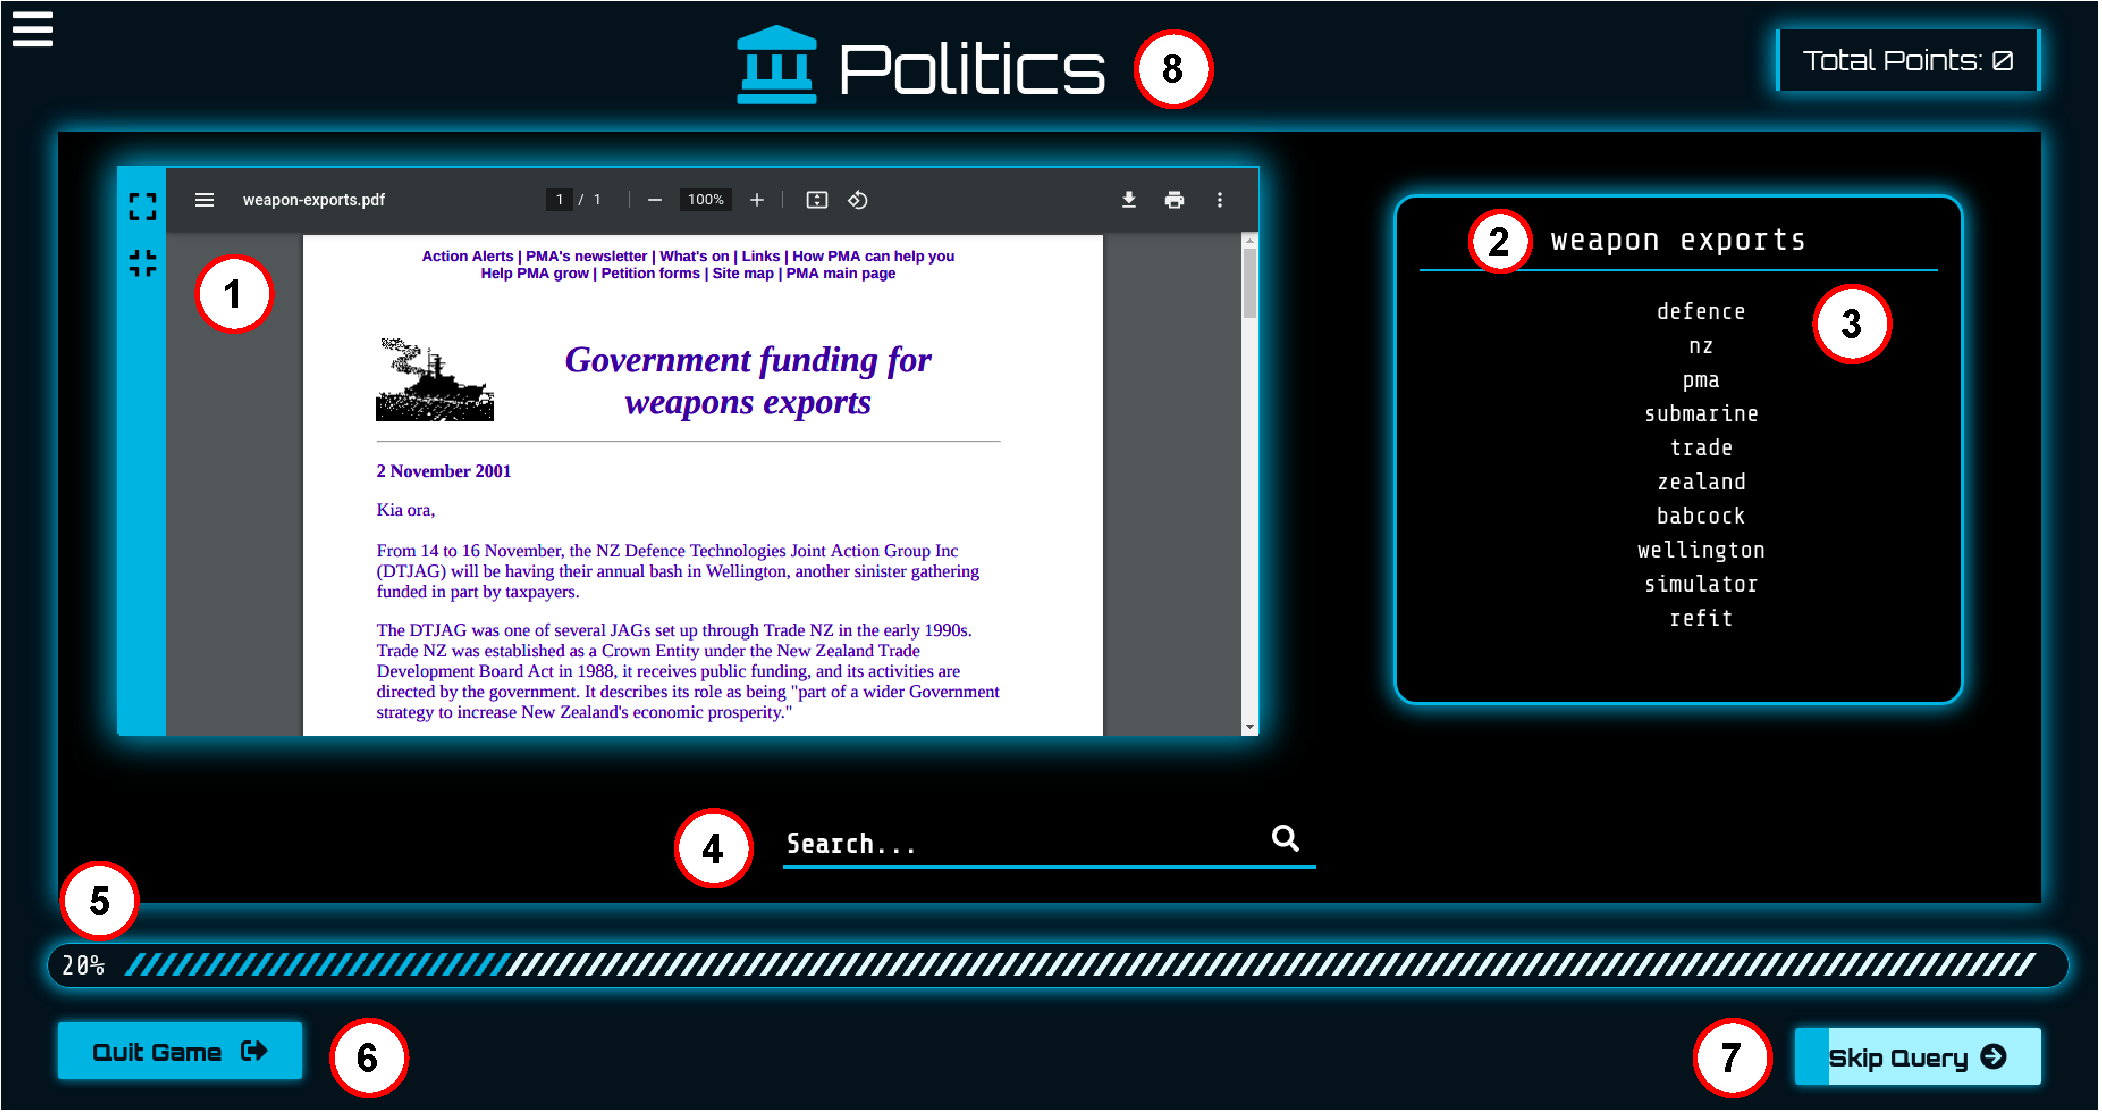
\includegraphics[width=1.0\textwidth]{graphics/game/game_description_all_elements.pdf}
    \caption{A screenshot of the main game interface, containing (1) the target document, (2) the associated query, (3) a list of auxiliary keywords, (4) a search field to enter queries, (5) a progress bar, (6, 7) buttons to skip a query or quit the game and (8) a header to show the selected category.}
    \label{fig:game_interface}
\end{figure}
In order to be able to go into more detail about the individual game elements, later on, we will briefly explain a typical game course in the following.\par
If users are playing for the first time, they get an introduction that describes the fictional scenario in which they find themselves. In this context, it is also explained what their task is and how they can solve it. Afterward, players get redirected back to the home screen, the starting point of the game. This home screen consists of a city map with different districts, each representing a different category (see Figure~\ref{fig:city}). Players may now start a new game by selecting a category and then clicking on the corresponding district on the map. The game interface will then open and participants can think of a suitable obfuscated query. If they submit an appropriate query, they get points and may continue the game or try to achieve more points.\\
In total, a game lasts five rounds. Once these are completed, players automatically are returned to the home screen. 
\begin{figure}[h]
    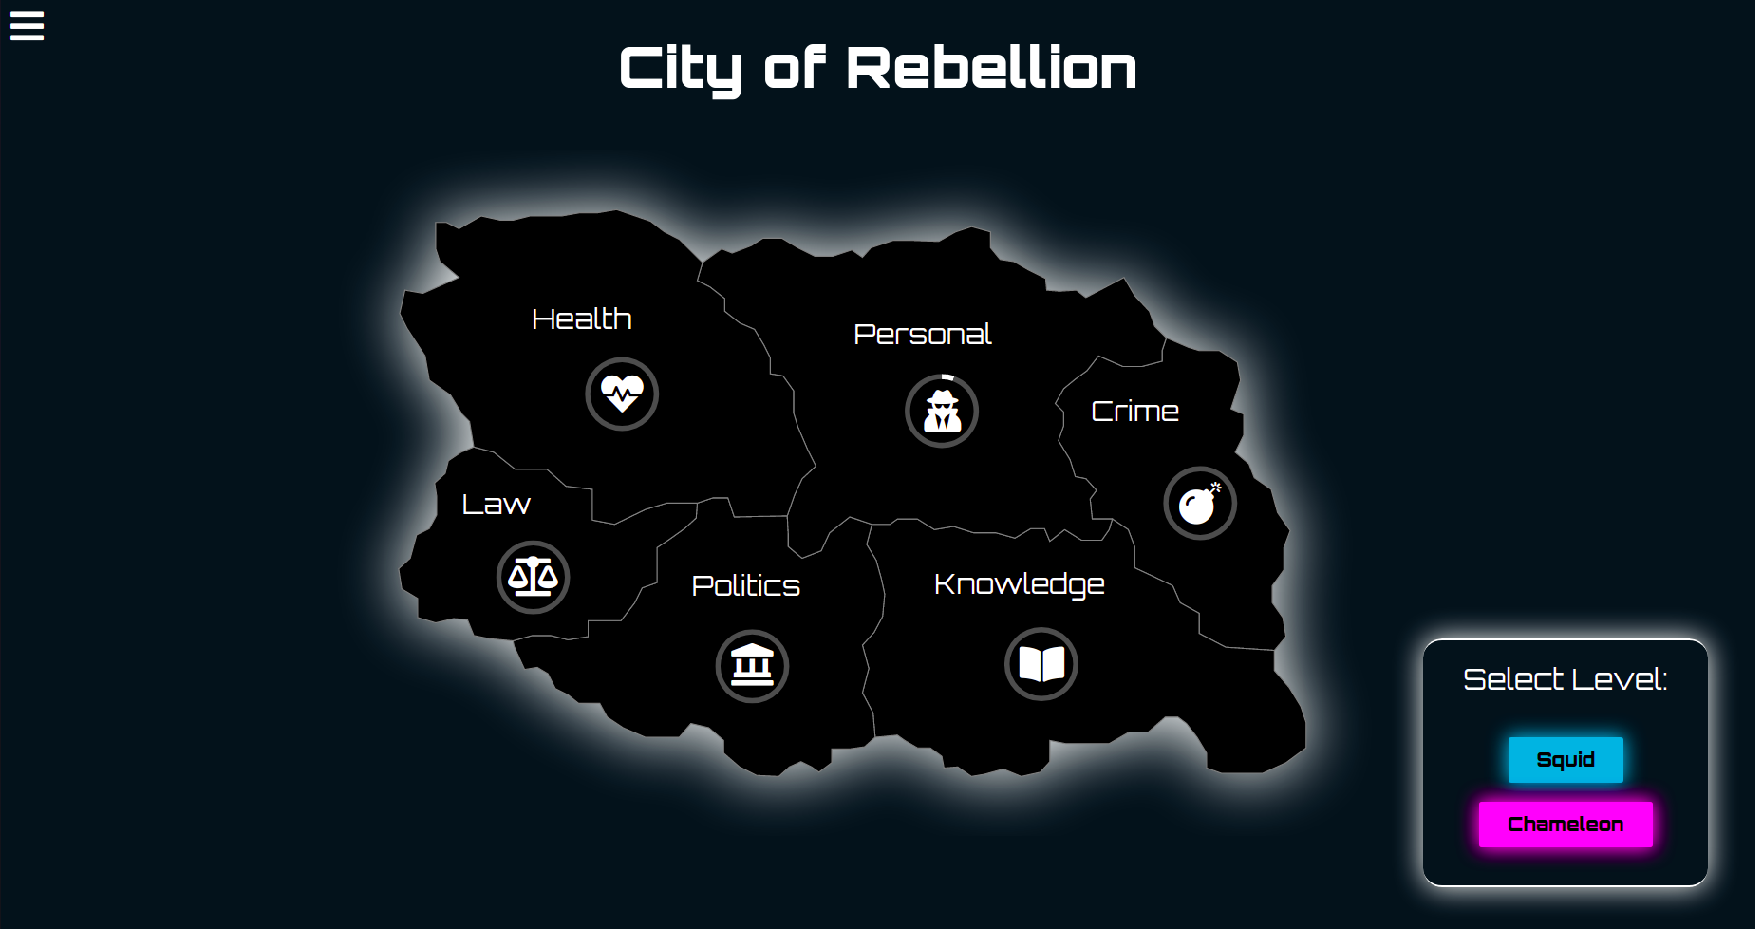
\includegraphics[width=1.0\textwidth]{graphics/game/city_levels.pdf}
    \caption{A screenshot of the game's home screen where players can click on a district of the city map to start a new game in the selected category.}
    \label{fig:city}
\end{figure}

\section{Game Properties}
\subsection*{Narrative}
To create a more meaningful experience, we thought of a background story for the game. The setting is a dystopia in which the government passed a law that completely abolishes data protection, turning the nation into a police state. The player takes on the role of a rebel in a resistance group. This group is helping others to hide their private information need by obfuscating queries before submitting them to a search engine.
This story is presented to users as a part of the game instructions and introduction (see Figure~\ref{fig:intro}).
\begin{figure}[h]
\centering
    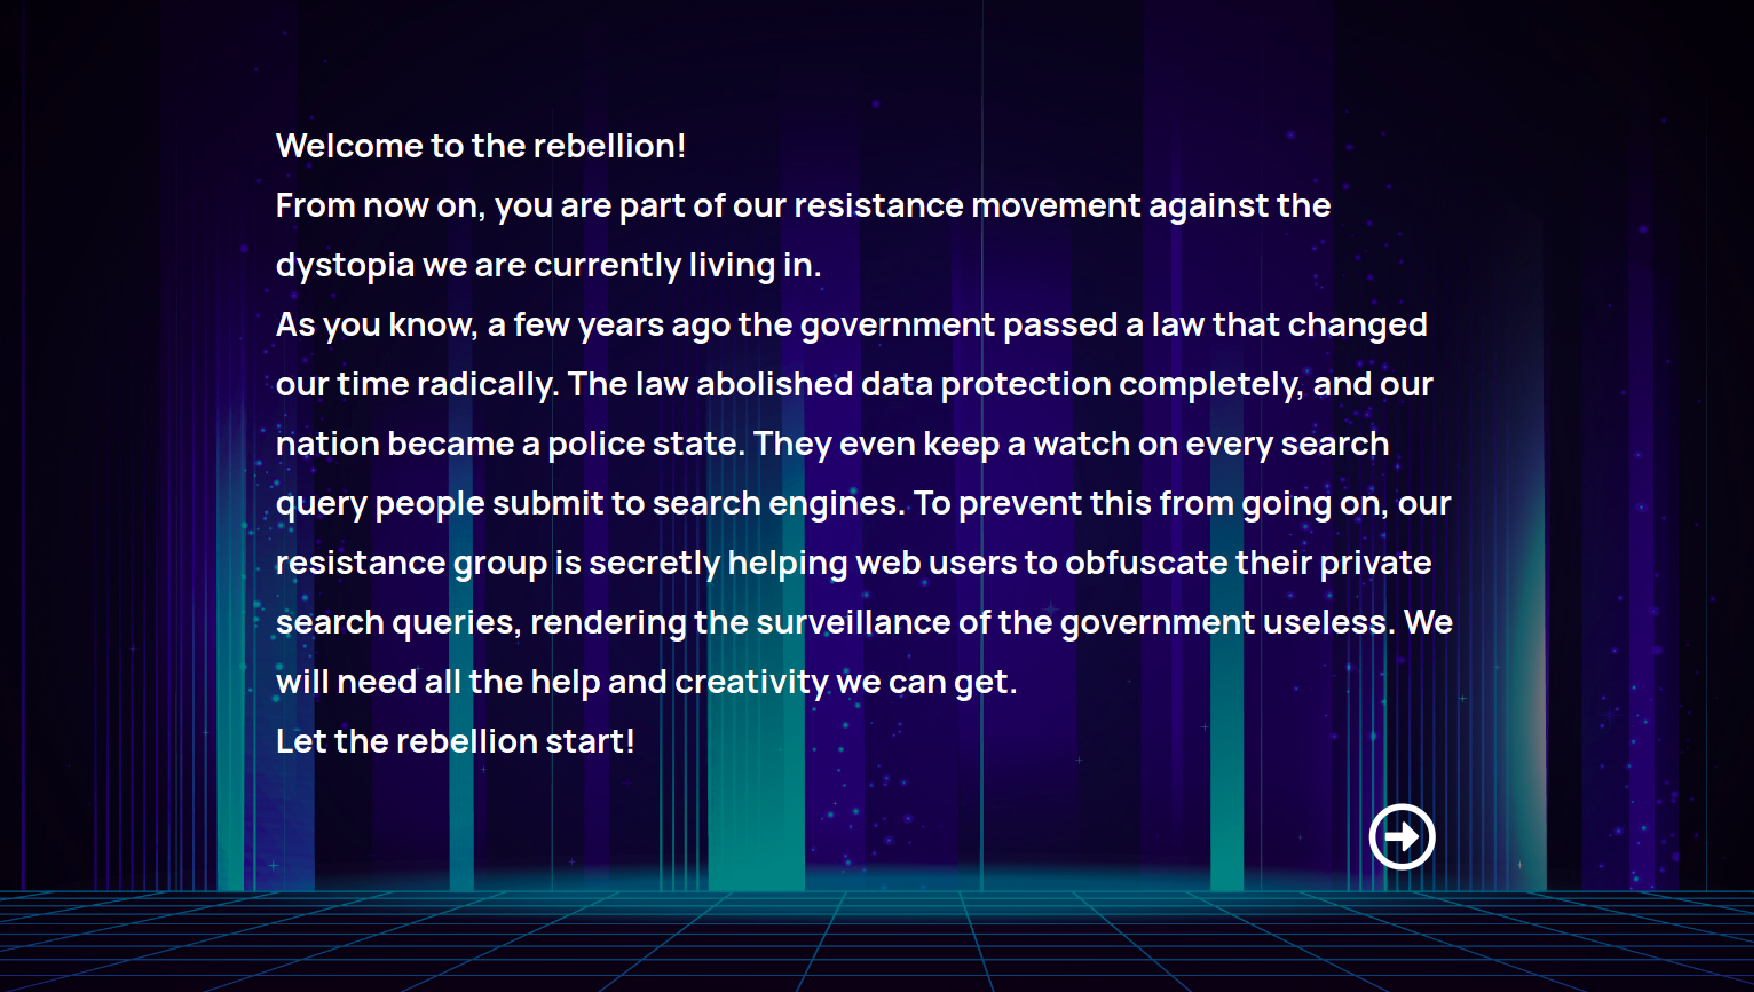
\includegraphics[width=1.0\textwidth]{graphics/game/introduction (1).pdf}
    \caption{A screenshot of the introduction that explains the background story of the game and the role of the player.}
    \label{fig:intro}
\end{figure}
This scenario is also reflected in the game design and structure. 
First of all, the starting point of the game is designed as a city map, which is supposed to represent the player's hometown and also serves as a starting point for a new game round (see Figure~\ref{fig:city}). The city makes things a bit more personal and at the same time offers a clear design for the categories which is in line with the story. In addition, the overall game design is futuristic to make the concept of a future dystopia more realistic.\par
With the help of an interesting scenario, we want to increase participation and the performance of players. For this reason, we have developed a background story that addresses the problem of search privacy and is linked to a widely known dystopian scenario. The emergence of a surveillance state, that collects profiles of all web users through their search queries, appears in many video games, books, and movies.
With this, we want to bring the motivation of this thesis closer to the users as well as create a recognition value and give players the possibility to immerse deeper into the scenario.

\subsection*{Levels}
Our game has two levels, Squid and Chameleon. The name givers of the levels are both animals that are masters of camouflage and thus reflect the task of players to obfuscate sensitive information needs. In the beginning, only the first level Squid can be played. When a player has successfully obfuscated five queries, a second level Chameleon gets unlocked (see Figure~\ref{fig:city}). The second level is more or less identical to the first, except for two small differences. First, the color scheme of the second level is purple in contrast to the blue Squid level. The second and critical difference is that now players will lose points if they use any auxiliary keywords. With this technique, we want to make sure that players have to become more creative in their obfuscation attempts. We also want to provide more variety to the game. Furthermore, adding levels to the game suggests progress to the players, creating a sense of acknowledgment.

\subsection*{Points}
Players receive points for successfully retrieving the target document while obfuscating the original query. The points are divided into different categories and are loosely based on some evaluation measures for information retrieval systems.
\begin{figure}[h]
\centering
    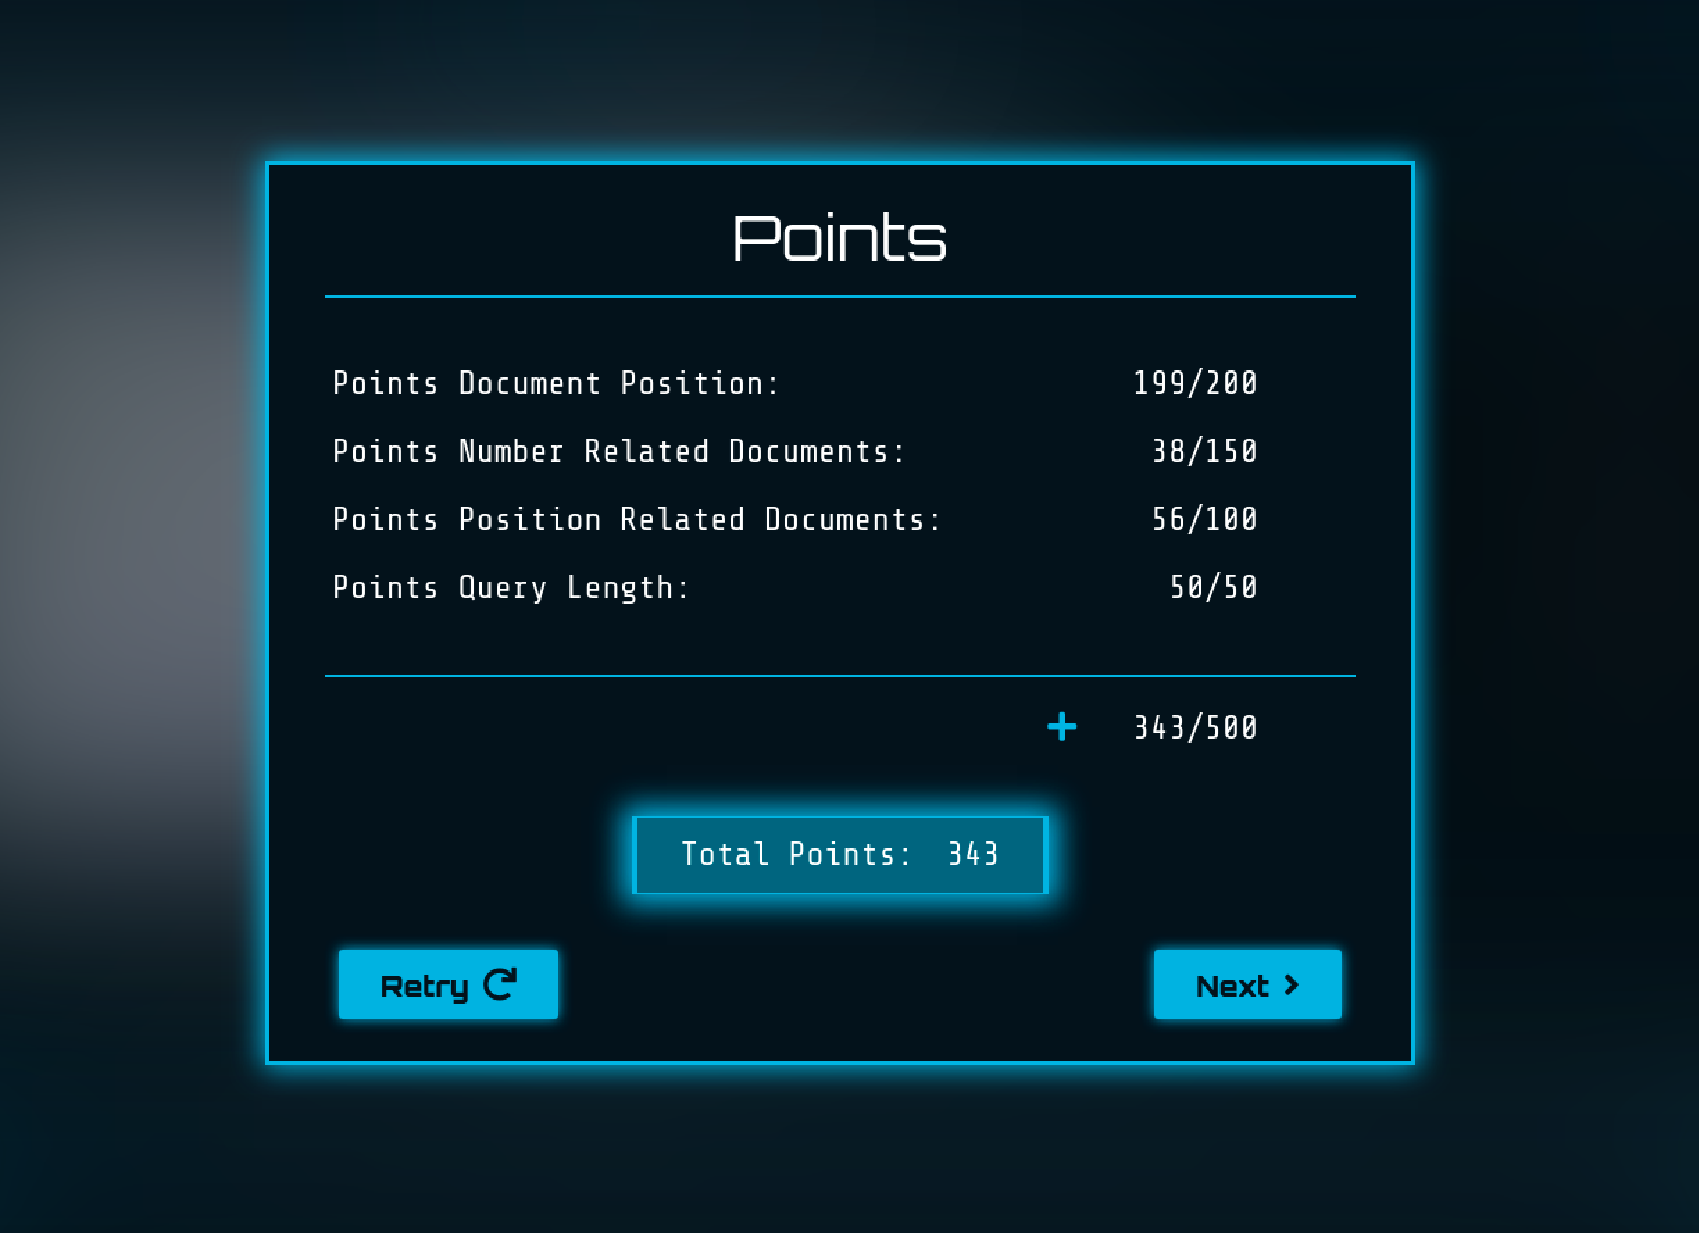
\includegraphics[width=0.8\textwidth]{graphics/game/points_cropped.pdf}
    \caption{A screenshot of the score board that opens up if a player retrieved the target document.}
    \label{fig:points}
\end{figure}
First of all, let's look at the points calculation of the first level Squid.
\newpage
\noindent Four factors play a role here:
\begin{enumerate}
    \item The position of the target web page inside the search response,
    \item the number of related documents that would also be retrieved if the original query were to be submitted,
    \item the average position of these related documents inside the response, and
    \item the length of the obfuscated query.
\end{enumerate}
Players could receive a maximum total of 500 points per round. First of all, it is checked whether the target document is among the top 8000 positions, which the search engine returns as soon as the player submitted his search query. If this is not the case, the player receive an error message and has to revise and resubmit his search query. If, however, the document was found by the search engine, the number of relevant documents, their average positioning, and the length of the player's search query are calculated. These variables are then used to calculate the corresponding points.\par
\begin{table}[t]
\centering
    \caption{(a) Steps of the algorithm to compute points for the position of the target web page. (b) Example of the points calculation for the average position of found related documents.}
    \label{tab:docpos}
\subfloat[Subtable 2 list of tables text][Target document]{
\begin{tabular}[t]{cc}
\toprule
Position & Points\\
\midrule
1 - 10&200\\    
11 - 20&199\\    
21 - 30&198\\ 
$\cdots$ & $\cdots$\\ 
101 - 120&190\\ 
121 - 140&189\\ 
$\cdots$ & $\cdots$\\ 
2001 - 2050&95\\ 
2051 - 2100&94\\ 
$\cdots$ & $\cdots$\\ 
5001 - 5100&35\\ 
5101 - 5200&34\\ 
$\cdots$ & $\cdots$\\ 
> 7000 & 10\\
\bottomrule
\end{tabular}}
\qquad
\subfloat[Subtable 3 list of tables text][Related web pages]{
\begin{tabular}[t]{cc}
\toprule
Average Position & Points\\
\midrule
x < 160 & 100 \\  
$161 < x \leq 320$  & 98\\ 
$320< x \leq 480$ & 96 \\ 
$\cdots$ & $\cdots$\\
\bottomrule
\end{tabular}}
\end{table}
For the web page's position (1.) a maximum of 200 points is possible. The further down the web page is positioned, the fewer points the player receives. To compute the final points, we divide the 8000 possible positions, on which the web page could be placed into steps, and, based on these steps, deduct points from the 200 starting points. In the range of the positions \mbox{1-100}, one point is deducted for every 10 steps down in the positioning, from \mbox{101-2000} it is 20 steps, from \mbox{2001-5000} 50 steps, from \mbox{5001-7000} 100 steps and from a positioning of 7001 and above players constantly receives 10 points as a minimum (see Table~\ref{tab:docpos}~(a)).\par
For the number of related documents (2.) players may reach 150 points at max. For this purpose, the number of relevant documents found is simply converted directly into points, for example, 24 found documents result in 24 points. Since we saved the IDs of 300 related documents for each query, players may retrieve more than 150. In this case, they simply get the maximum of points (see Table~\ref{tab:docpos}~(b)).\par
The third factor (average position of related documents) brings a maximum of 100 points. The computation is similar to the calculation of the points that players can achieve for the positioning of the target web page. For this purpose, the 8000 positions that the search engine returns as a maximum are divided into levels of 160 positions each. For each level down, which means a worse positioning, two points are deducted from the initial 100 (see Table~\ref{tab:docpos} (b)). For example, if the average position is $\leq$ 160, players receive 100 points, if it is between 161 and 320, 98 points are awarded, and so on.\par
And finally, players get points for the query length. The maximal number of points users can achieve here is 50. Players receive the maximum number of points if their query is shorter or the same length as the original query. For each additional word, one point is deducted. In this context, length is defined as the number of words the query consists of.\par
In the second level Chameleon, the same aspects play a role in calculating the points. This means that players receive points for the same criteria as before. In addition, however, the use of the suggested keywords has a negative effect on the achievable points. When players use one or more of the provided keywords, they lose points. This works as follows: Each keyword has a certain value, which is reflected by its position in the list. The value decreases with each word in descending order. Thus, the first word is worth 100 points, the second 90, and so on. When a player submits a query, the values of the keywords used for it are summed up and then subtracted from the total number of points. This means that players can lose up to 550 points which would result in a negative score. We implemented this kind of point calculation to encourage the players to give more thought to the formulation of their search queries. 

\subsection*{Performance Graphs}
In contrast to the competitive leaderboards, performance graphs show the individual performance of players. This can create a sense of mastery for the participants, motivating them to invest more time in the game \cite{wirkungGamificationBuch}. We implemented two kinds of graphs. One kind shows the performance of users (collected points and number of successfully obfuscated queries) over time (see Figure~\ref{fig:statistics}. The second kind shows how many queries have already been solved in each category.
\begin{figure}[h]
    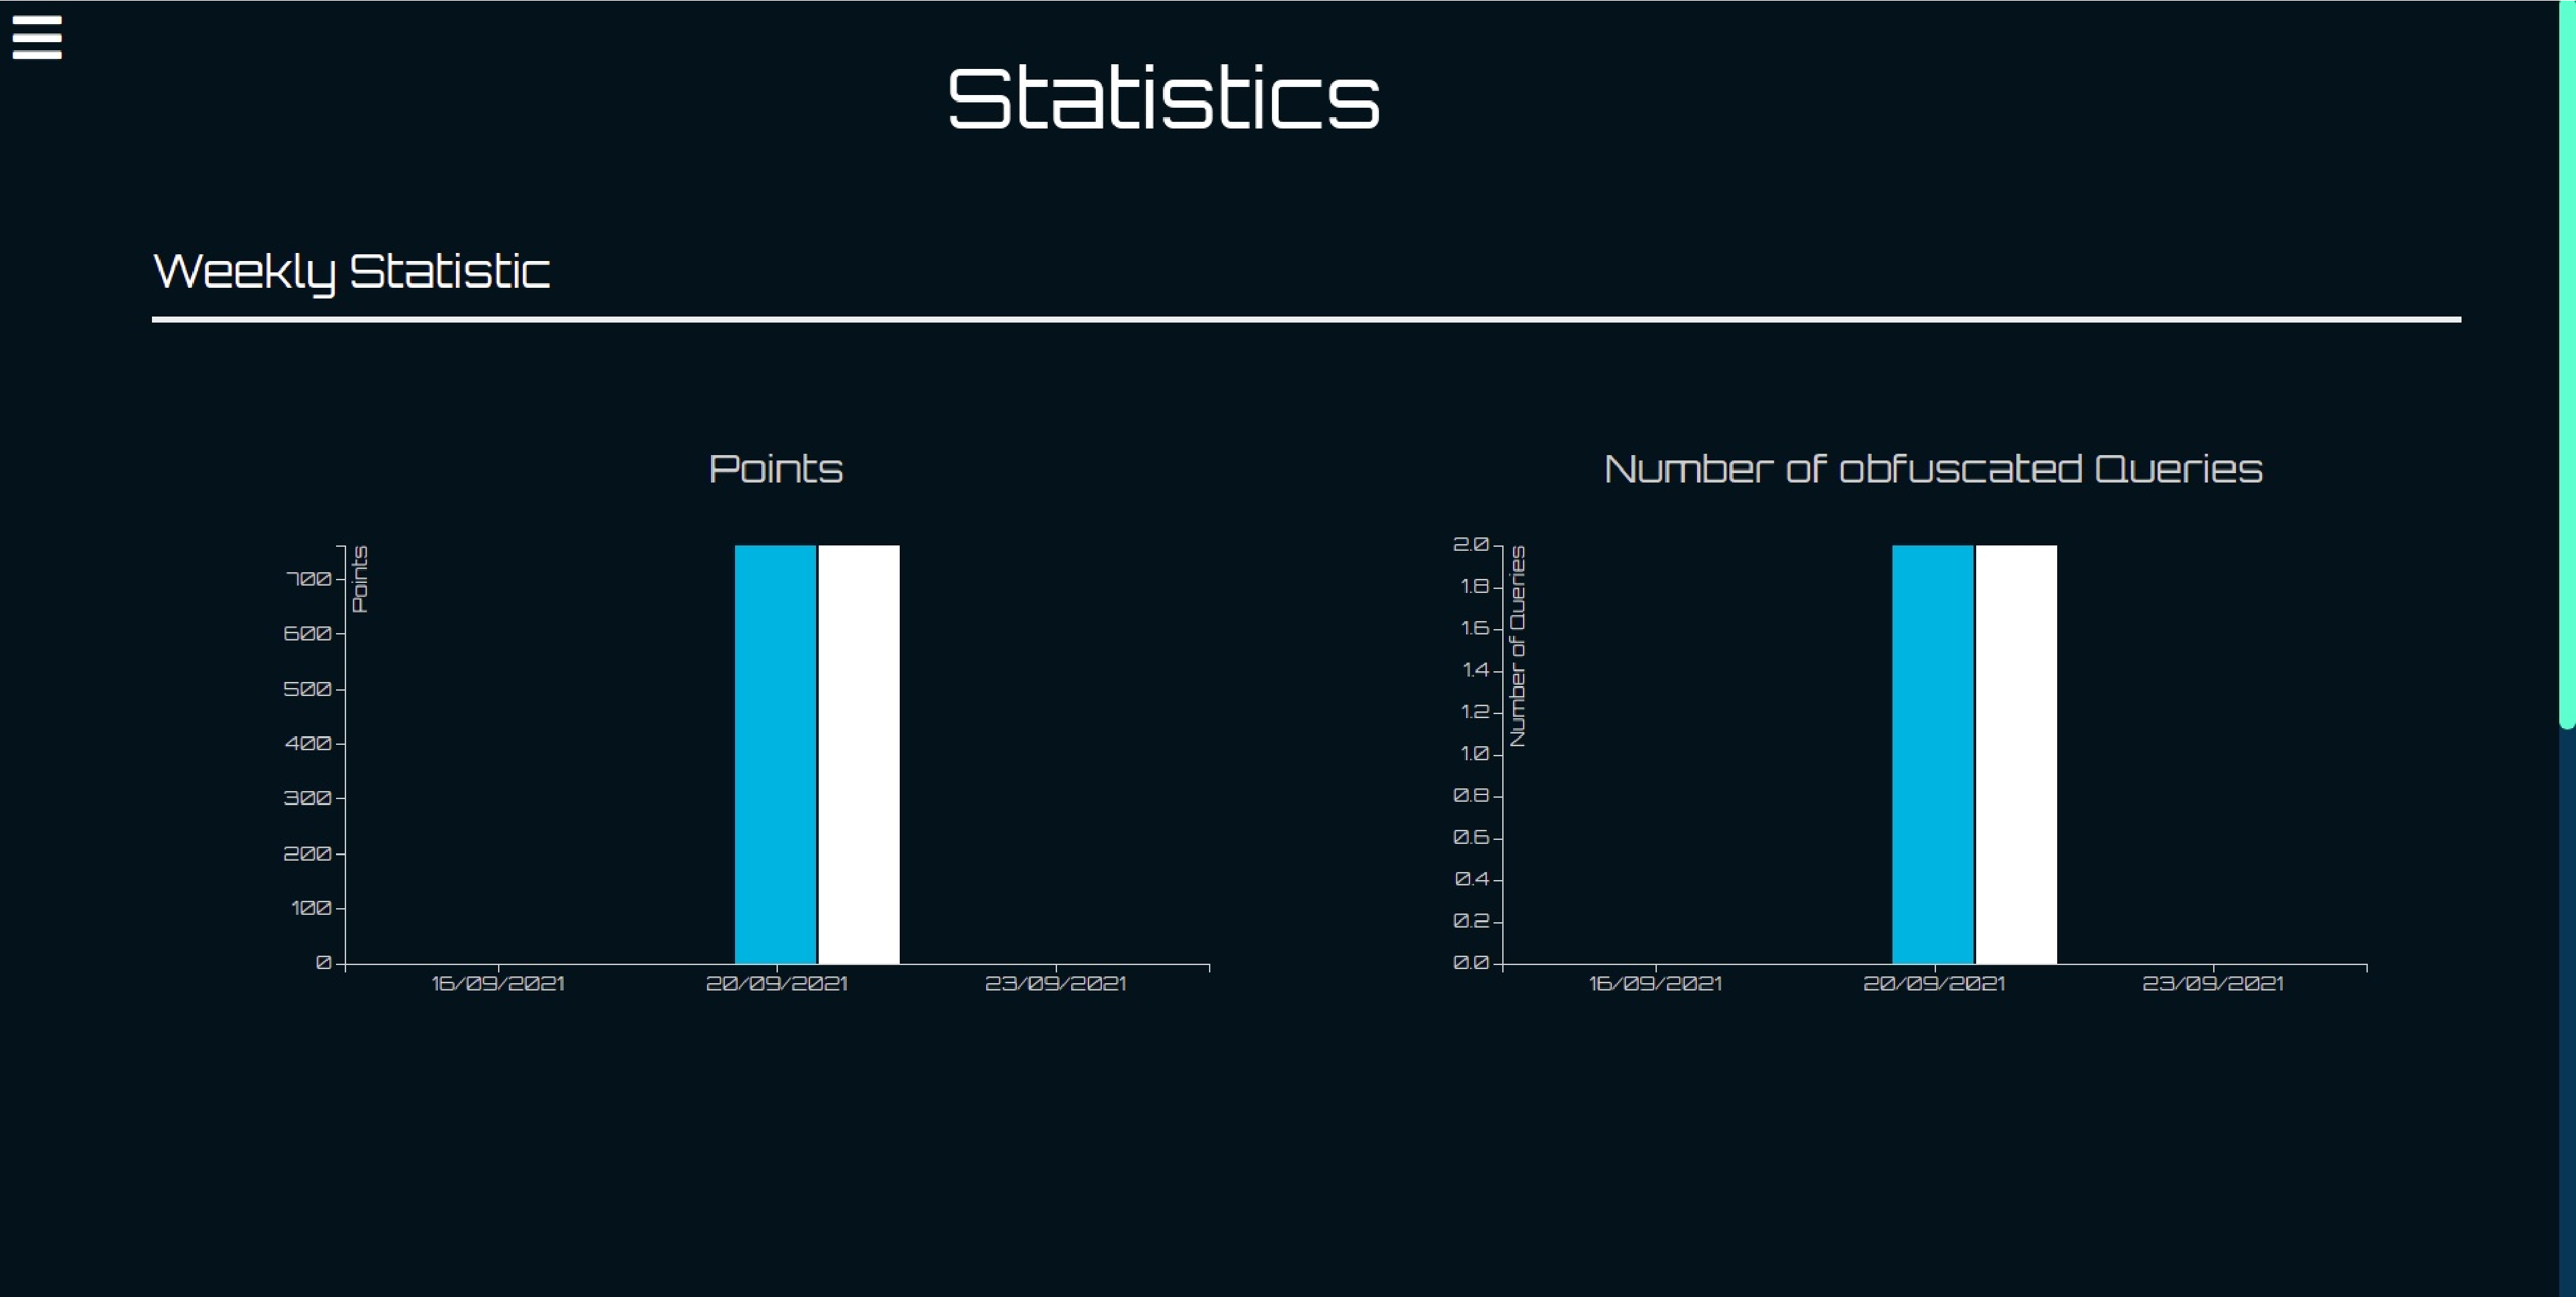
\includegraphics[width=1.0\textwidth]{graphics/game/statistics.pdf}
    \caption{A screenshot of a user's performance graphs. One graph (left) shows how many points a player received for each level and in total for every day he or she played. The other graph (right) shows how many queries the player successfully obfuscated over time.}
    \label{fig:statistics}
\end{figure}

\subsection*{Usernames}
When a participant visits the web page of the game for the first time, a new entry in our MongoDB database is created with a random user name. This username consists of an adjective followed by a surname. It is used to identify a player inside the leaderboards and can be changed to fit the player's preferences (see Figure~\ref{fig:username}). The username is a game design element that creates more freedom for players as well as customization.
\begin{figure}[h]
    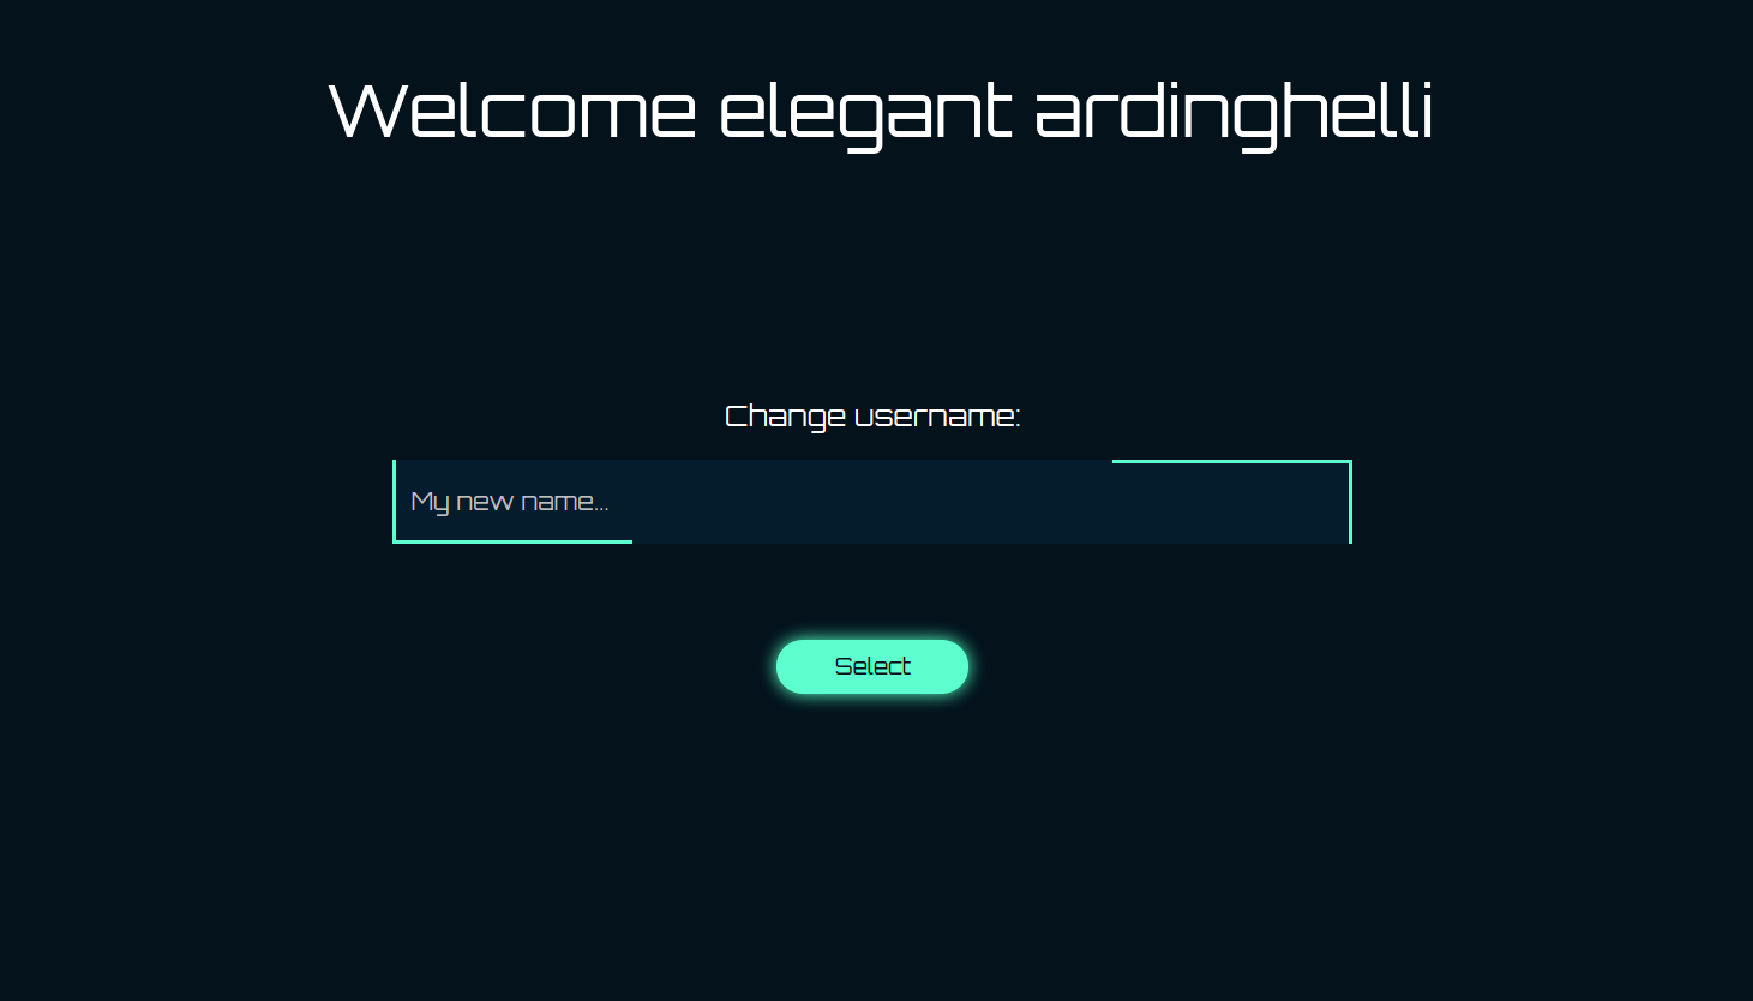
\includegraphics[width=1.0\textwidth]{graphics/game/username (1).pdf}
    \caption{A screenshot of the form which allows players to choose their own usernames.}
    \label{fig:username}
\end{figure}

\subsection*{Leaderboards}
We have designed three leaderboards, one for each level and a third one that combines the points from both levels to an overall performance (see Figure~\ref{fig:leader}). With this, we want to achieve a sense of challenge between the users and motivate them to climb to the top by playing more and/or better than the others. We designed three leaderboards to prevent the demotivating effect one could have. Now, players have a greater chance to be at the top of at least one of the boards. Furthermore, participants can gain a lot of points in a short period which makes it easier to raise inside this hierarchy. We added this game design element to help us to increase the user performance, thus, collecting more data.
\begin{figure}[h]
    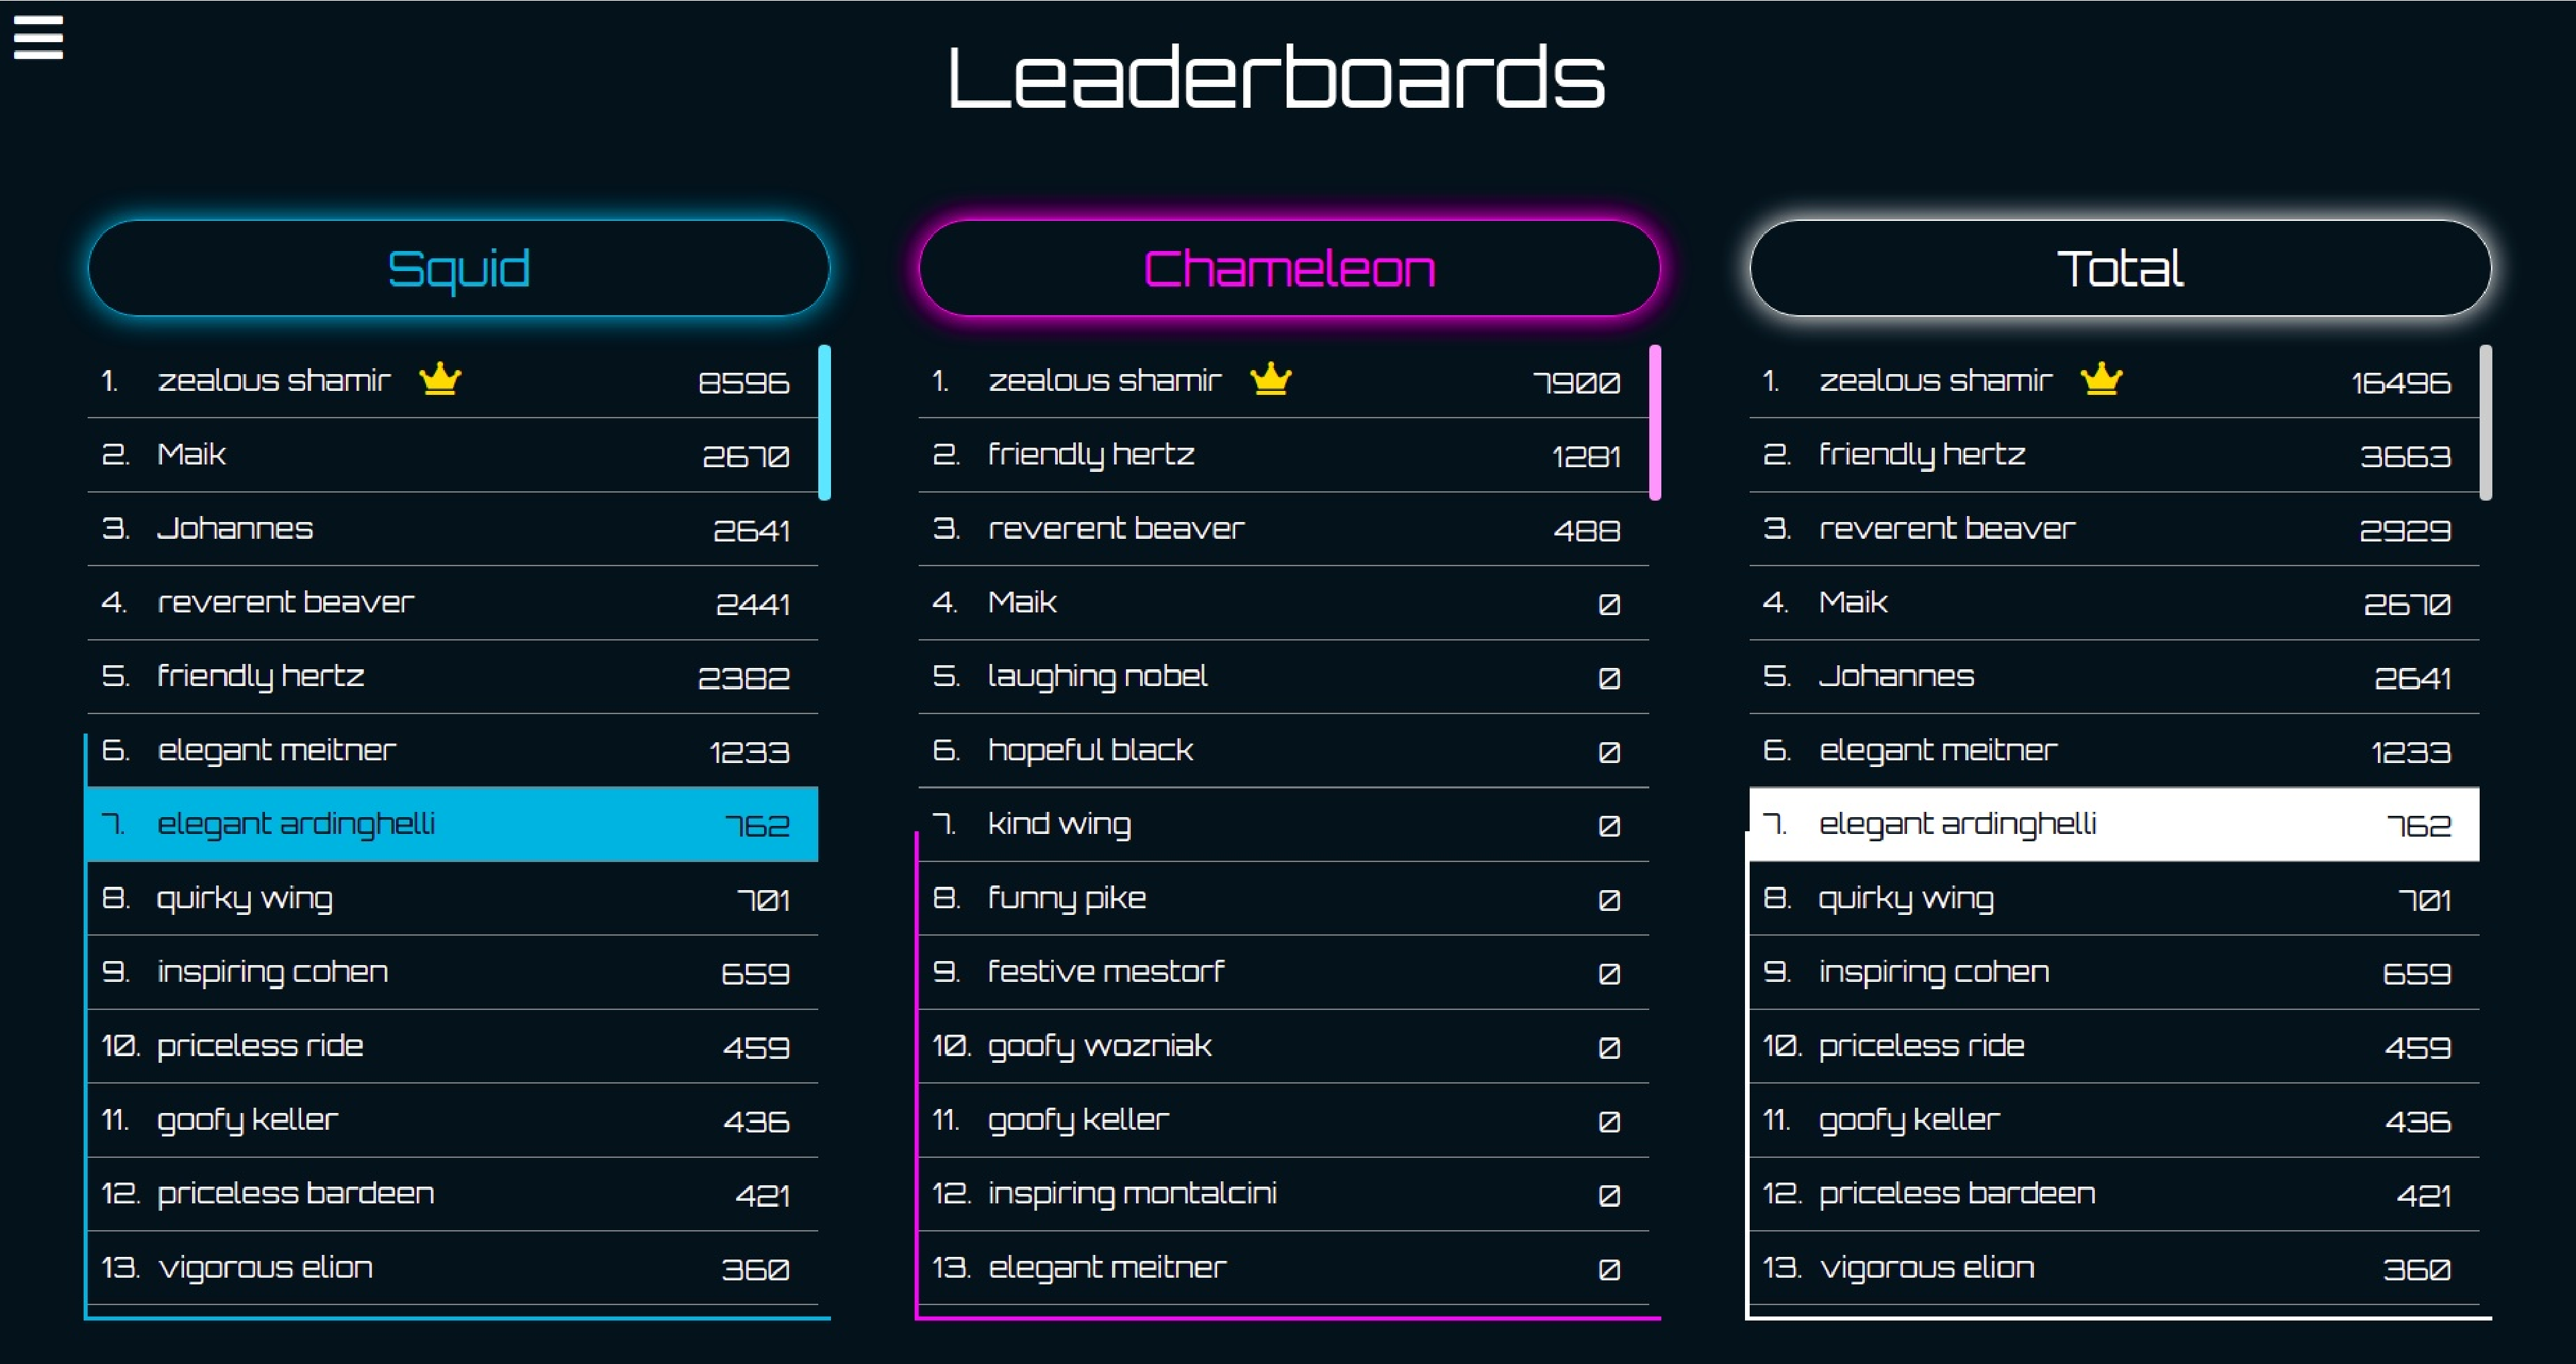
\includegraphics[width=1.0\textwidth]{graphics/game/leaderboards.pdf}
    \caption{A screenshot of the three different leaderboards, one for each level and one for an overall performance.}
    \label{fig:leader}
\end{figure}

\subsection*{Categories}
To make things more interesting and to create more freedom of choice, players may choose between six categories of query types. These categories correspond to specific subject areas into which the queries could be classified, namely Health, Personal, Crime, Knowledge, Law, and Politics (see Figure~\ref{fig:city} and Table~\ref{tab:category}). This potentially has a positive effect since players may choose to play game rounds in a category they are either interested in or have further knowledge about~\cite{gamifiedSearch}. This offer makes the game more interesting and diverse since it creates meaningful choices and demonstrates preferences. It is a game technique that addresses the feeling of empowerment and the creativity of players~\cite{actionableGamification}, thus, satisfying psychological needs.

\subsection*{Progress Bar}
We implemented two different kinds of progress bars in the game.
One kind of progress bar is part of the main game interface and indicates in which game round a player currently is (see Figure~\ref{fig:game_interface}). It acts as a simple feedback function that reflects the player's status. Furthermore, it serves as a goal and motivates people to finish the game round by addressing the psychological need to finish incomplete things \cite{actionableGamification}. The other progress bar is part of the home screen included in the city map. On this map, a donut chart is drawn for each category, showing how many queries from that category have been successfully obfuscated (see Figure~\ref{fig:category1}, \ref{fig:category2}) in the selected level.
\begin{figure}[ht!]
    \begin{minipage}[b][][b]{0.46\textwidth}
    \centering
    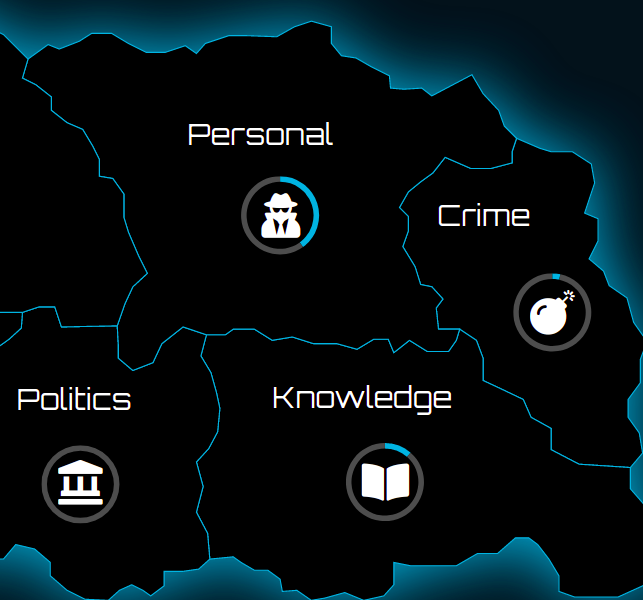
\includegraphics[width=0.9\textwidth]{graphics/game/city_category.png}
    \caption{A screenshot of the category graphs in the level Squid.}
    \label{fig:category1}
    \end{minipage}
    \hfill
    \begin{minipage}[b][][b]{0.46\textwidth}
    \centering
    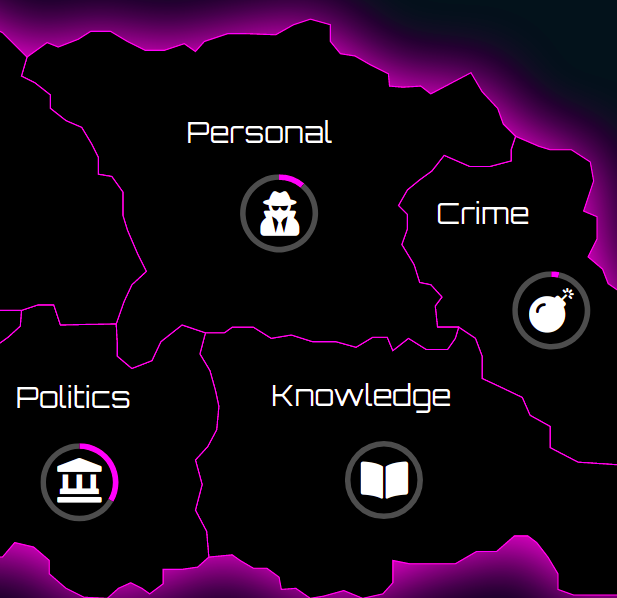
\includegraphics[width=0.87\textwidth]{graphics/game/city_category_2.png}
    \caption{A screenshot of the category graphs in the level Chameleon.}
    \label{fig:category2}
    \end{minipage}
\end{figure}

\subsection*{Other Features}
We implemented a few more features that are not directly typical game design elements but also help to make the user experience more pleasant. To prevent frustration and make the navigation inside the game easier, we added two buttons in the main game interface. These buttons allow the players to either quit the game and return to the home screen or to skip a query after 60 seconds if they get stuck (see 6. and 7. in Figure~\ref{fig:game_interface}). Another feature is the Retry button. Every time, players successfully obfuscated a query they get the possibility to continue with the next query or try to improve their current score. The idea behind this button is to give players the chance to improve their performance. The auxiliary keywords were taken from the list of keywords that the search engine ChatNoir~\cite{chatnoir} extracted for the corresponding web page.

\section{Game Development}
In this section, we explain the different components of the game development by describing the process of collecting queries to obfuscate and rendering the target documents visually appealing. Afterward, we describe how and what data we collected for the evaluation.

\subsection{Sensitive Queries}
The first step we had to take was to create a collection of sensitive search queries. For this purpose, we consulted the AOL query logs, a collection of TREC Web track queries~\cite{anserini}, and a paper of Arampatzis et al.~\cite{arampatzis} from which we extracted suitable sensitive queries. The basis of our collection is a list of sensitive queries that Arampatzis et al. created \footnote{\url{http://lethe.nonrelevant.net/datasets/95-seed-queries-v1.0.txt}}. However, we skipped all queries with sexual or inappropriate content like \texttt{free porn movies}. These kinds of queries are certainly sensitive and should stay private but their content is unsuitable for our game, especially since we display relevant web pages. Skipping these unsuitable queries, allowed us to gather 82 queries for our collection out of the original 95. Furthermore, we extracted queries from a collection of sensitive TREC Web Track queries. These queries were particularly helpful for our evaluation since there exist annotated data on the information needs and relevant web pages. With this additional data, we are able to make even more well-founded statements about the obfuscation skills of players. The biggest sources for our collection are the AOL query logs, a huge collection of queries from various users. Here, we also ignored the pornographic and hateful contents. Additionally, inspired by these resources, we added some self-devised queries to our collection.
Overall, we assembled a list of 700 sensitive search queries. To group the queries into districts on the city map, we had to find suitable categories for the queries. Inspired by Arampatzis' paper \cite{arampatzis} and our list, we were able to derive six different categories in which we organized the queries (see Table~\ref{tab:category}).

\newpage
\begin{table}
\centering
\caption{The six different categories in which we organized the queries and the number of queries for each category.}
\label{tab:category}
\begin{tabular}[th]{ccc}
\toprule
Category & Example Query & Number of Queries\\
\midrule
Health & \texttt{folk remedies sore throat} & 65\\    
Personal & \texttt{cheating husbands} & 45\\    
Knowledge & \texttt{evidence for evolution} & 35\\ 
Crime & \texttt{forged passports} & 30\\ 
Law & \texttt{pregnancy discrimination laws} & 15\\ 
Politics & \texttt{weapon exports} & 15\\ 
\bottomrule
\end{tabular}
\end{table}

\subsection{Visual Enriching of Sensitive Documents}
\label{enriching}
To support users in obfuscating queries, we show them a relevant ClueWeb document for the sensitive query. For this task, we used the Elasticsearch-based search engine ChatNoir, a search interface for the two ClueWeb corpora and the Common Crawl~\cite{chatnoir}. It was developed especially for research purposes and has a freely accessible API~\cite{chatnoir}, allowing us to easily access the ClueWeb12 from which we chose the target documents for the sensitive queries. We decided to use the ClueWeb12 since web pages from 2012 often look better than those from 2009. This improves the graphic aesthetics of our game. Moreover, modern-looking web pages are more compliant with our futuristic background story. ChatNoir also provides additional data for each web document, such as a list of keywords, which we have adopted for the game (see Section \nameref{overview}). However, documents in the ClueWeb are not intended to be shown to humans because additional resources like CSS stylesheets or images are not included in the crawl. This means that most web pages are not well-formatted and are rather unsightly and chaotic. That would be disadvantageous for our game because you can not draw information from these documents easily. To counteract this issue, we have developed a strategy that allows us to make web pages visually pleasing again with the help of the web archive Wayback Machine. This works as follows (see Algorithm~\ref{alg:resources}):\par
First, we send a request to ChatNoir that returns the corresponding top three web documents. For each document, we extract the original URI and the time at which it was crawled. With these two pieces of information, we send a request to the Wayback Machine API. The response then tells us whether the web page exists inside the web archive or not. If the web page is not inside the archive, the algorithm repeats the process described above with the next document. Otherwise, we take the URL of the web page inside the Wayback Machine. Since there can exist several snapshots of the same web page inside the web archive, we save the URL of the version that was crawled in close temporal proximity to the wanted ChatNoir document. Next, we replace the links to the stylesheets and images in the ChatNoir document so that they point to the resources stored by the Wayback Machine. Therefore, we first extract all stylesheet links from the web page inside the Wayback Machine. This is done with the Python library Beautiful Soup and the URL we got from the web archive in the previous step. Next, we extract the stylesheet links from the ChatNoir web page and delete the part of the links that define the communication protocol. Afterward, we check for all stylesheet links of the ChatNoir web document if they are part of a web archive link. If this is the case, then the link inside the ChatNoir web page gets replaced by the link of the Wayback Machine. Afterward, the same is done for the image resources. In the last step, the changed ChatNoir web page is saved as a new HTML file.\\
We also deleted all links of the \texttt{<a>} tags from the file to prevent users from being redirected when they accidentally click on one of them.
\begin{algorithm}[t!]
	\caption{Change Resources}\label{alg:resources}
	\hspace*{\algorithmicindent} \textbf{Input:} Set Q of sensitive search queries \\
    \hspace*{\algorithmicindent} \textbf{Output:} HTML files with changed resources for queries in Q
	\begin{algorithmic}[1]
		\For {q in Q}
		    \State chatnoir\_response = request\_top\_3\_documents(q)
		    \For {document in chatnoir\_response}
		        \State archived\_document = closest\_snapshot\_in\_archive(document.uri, 
		        \State \hspace{9.7em} document.timestamp)
		        \If {archived\_document is not None}
                    \State replace\_stylesheets(document, archived\_document)
		          %\State{\# does the same exchange of links for the images}
		          \State replace\_images(document, archived\_document) 
		          \State render\_enriched\_document(document)
		          \State save(document)
		        \EndIf
		  \EndFor
	    \EndFor
	\end{algorithmic} 
\end{algorithm}

\newpage
\subsection{Selection of Queries}
Finally, we had to decide which queries should become part of our game. For the selection process three criteria were taken into consideration:
\begin{enumerate}
    \item The target document is part of the web archive.
    \item The resources of the target document could be enriched enough to be visually pleasing.
    \item The target document is relevant for the sensitive query.
\end{enumerate}
First of all, if neither of the top three documents of a query was found inside the web archive, then the query was considered to be unsuited. That is because the look of a web page is important for the game (see Section \nameref{enriching}). Next, we had a look at all queries for which at least one of the top web pages could be visually enriched. Not all web pages could be restored by our algorithm and were therefore unsuited to be part of the game. The last criterion for a query or rather a web page was if it contains relevant and helpful data that could support the players in their obfuscation attempts. Only if at least one of the web pages for a query met all these criteria, the query was included in our game. This selection process was very strict and only 50\% of the regarded queries passed it. After the completion of this process, the selected documents were converted and saved as PDFs. The reason for this conversion was the fact that the web pages needed a long time to load which was rather disadvantageous for the usability of our game. In addition to the mentioned criteria, we had to make sure that enough queries for each category remained. In total, 200 queries were selected for the game.

\subsection{Sampling}
In our first prototype, we included ChatNoir as the search engine. But through testing, we realized that obfuscating queries while still retrieving relevant web pages can be difficult. We became aware that one problem is the large number of documents inside ChatNoir (638.8m alone in the ClueWeb12). The size of this corpus made it hard to find the target web pages without using terms from the original query. Therefore, we took a sample consisting of 626.629 ClueWeb documents and built an index.
First, we had to make sure, that all needed web documents would be part of the sample. For this reason, we sent a request to ChatNoir for every query of the game and some randomly selected queries from our collection. From every response, we saved the top 1000 web pages. For more variety, we used the sampling strategy of Aramatzis et al.~\cite{arampatzis} to add random documents to our sample. This idea works as follows. First, the query \texttt{www} is submitted to a search engine (in our case ChatNoir). The top result is added to the sample which is then used to select a new random query. This process is repeated until the desired amount of web documents is acquired. In the last step of our sampling process, all collected web documents were stored in a file. Then we transformed the raw HTML of each document into its text by using the parsing library Jsoup.\par
With the prepared data, we were able to build an index with Pyserini, a Python interface for the Ansirini toolkit. This index served us as a smaller search engine alternative to ChatNoir. The advantage of using Anserini~\cite{anserini} is that it uses a similar retrieval model to ChatNoir (BM25, BM25F for ChatNoir). This allows us to draw conclusions about the query obfuscation skills of humans in the context of a bigger search engine. 

\subsection{Logging}
For our evaluation, we had to collect data on the obfuscated queries. Therefore we used logging. Every time a new sensitive query is presented to players in a game round, their ID, the sensitive query, the timestamp, and the category and level they are playing in, are saved inside a log file. Furthermore, in addition to the previously mentioned data, the obfuscated queries of users are stored as soon as they submit it. Hereby, each user-specific log entry is designed as a Python dictionary so that the entries can be combined into one JSON file for the evaluation later on. This is what typical log entries look like:
\begin{small}
\begin{lstlisting}[language=json,firstnumber=1]
{
    "_id": "eb605791-c99f-4ff7-a900-4817da86925e",
    "username": "cool euclid",
    "category": "knowledge",
    "original query": "usda food pyramid",
    "level": "squid",
    "timestamp": "Tue Oct 12 09:50:24 2021"
}
\end{lstlisting}
\begin{lstlisting}[language=json,firstnumber=1]
{
    "_id": "91f173db-f26c-4d97-8d27-a5fb05aed3e7",
    "username": "strange spence",
    "category": "personal",
    "original query": "bankruptcy",
    "user query": "no money",
    "level": "chameleon", 
    "timestamp": "Tue Oct 12 12:50:30 2021"
}
\end{lstlisting}
\end{small}

\subsection{Preprocessing the Log File}
We use the collected and prepared log data to analyze the efficiency and effectiveness of players in obfuscating sensitive information needs. We research how long players needed to formulate an obfuscated query, what kind of terms they used, at which position they retrieved the target document and the number of retrieved related web pages, etc.. To make profound statements about these aspects that we use as a mean to determine the effectiveness and performance of players, the log data needs to be prepared and amended first. Therefore, we wrote a Python script that generates data for each obfuscated query.\par
First, we analyze the efficiency of players that we define as the time they spend to obfuscate a sensitive query. For this, we collect all entries from the log files that have the same user ID and refer to the same sensitive query. We then sort these entries by their timestamp and calculate the time spans between them. This gives us the seconds needed for each obfuscated query.
Next, we check for each submitted query if it contains one or more of the provided keywords. We save which of the suggested keywords were used and how many. Then, we measure the effectiveness of the obfuscated query by submitting it to ChatNoir. The response is then stored in a shortened version, which contains only the ID, the TREC ID, and the score for each retrieved web document. This response is then further used to determine the position of the target web page, the number of related documents, and their average position. This process is performed for the ClueWeb09, the ClueWeb12, and our document sample.
We chose to analyze the effectiveness of players for the sample as well as for ChatNoir so that we could research how much the size of a document collection would influence the effectiveness of the players' queries. Furthermore, this data could help to analyze the success rate of users. This could be used as an indicator if players get frustrated because the game is too difficult.
Finally, we test whether the users have used terms from the target document in their queries. For this, we first convert the content of the target web page into human-readable text with the Python library Beautiful Soup. Then we use a tokenizer for the query and the web page text, remove all stopwords and apply the porter stemmer from NLTK. We do this to make the web text comparable to the query so that we may check if it contains terms from the web document. Next, we check for each word in the revised query if can be found inside the web page text. Through this process, we save which of the words were used and how many. In a final step, we check if players used words or phrases from the target document in or as their queries. Therefore, we convert the tokenized query and the web page text back to one string each by separating every word with a space. Then we check whether the obfuscated query is a phrase from the web page or not.
\chapter{Evaluation}
In this chapter, we evaluate the prepared log files of our game to study the effectiveness and efficiency of the obfuscated queries. We have a look at some general aspects like the distribution of the obfuscated queries among players and their preferences regarding the categories and levels. Then we compare the average length of queries formulated by the participants with the length of the sensitive queries. We also investigate the overall success rate (target document retrieved) of players and the Mean Reciprocal Rank of the participants' queries in our document sample and ChatNoir. Finally, we categorize the obfuscated queries into five different types and compare their effectiveness to each other and to queries automatically obfuscated with the approach of Arampatzis et al.~\cite{arampatzis}.\par
We recruited users for our query obfuscation game from an information retrieval course and dedicated mailing lists at our universities (Bauhaus Universit{\"a}t Weimar, Martin-Luther-Universit{\"a}t Halle-Wittenberg). The information retrieval course was held at the Martin-Luther-Universit{\"a}t Halle-Wittenberg ($\approx$ 20 students). As a result, we were able to acquire 72 players which submitted a total of 1.534 obfuscated queries, 1.476 of those unique. 38 of the players completed a demographic survey which revealed that 13 were female, 25 male and their age ranged from 19 to 64 years.\par
There is great variance among the players regarding the number of their obfuscated queries. About 42\% of the players only submitted one to five queries and about 18\% submitted six to ten. This means that most players ($\approx$ 60\%) played one or two game rounds. As we can see in Figure~\ref{fig:distribution:num:queries}, the number of participants who submitted more than ten queries declines with increasing query quantity. However, we had one very engaged player who alone submitted a total of 499 obfuscated queries.  
\begin{figure}[h]
    \centering
    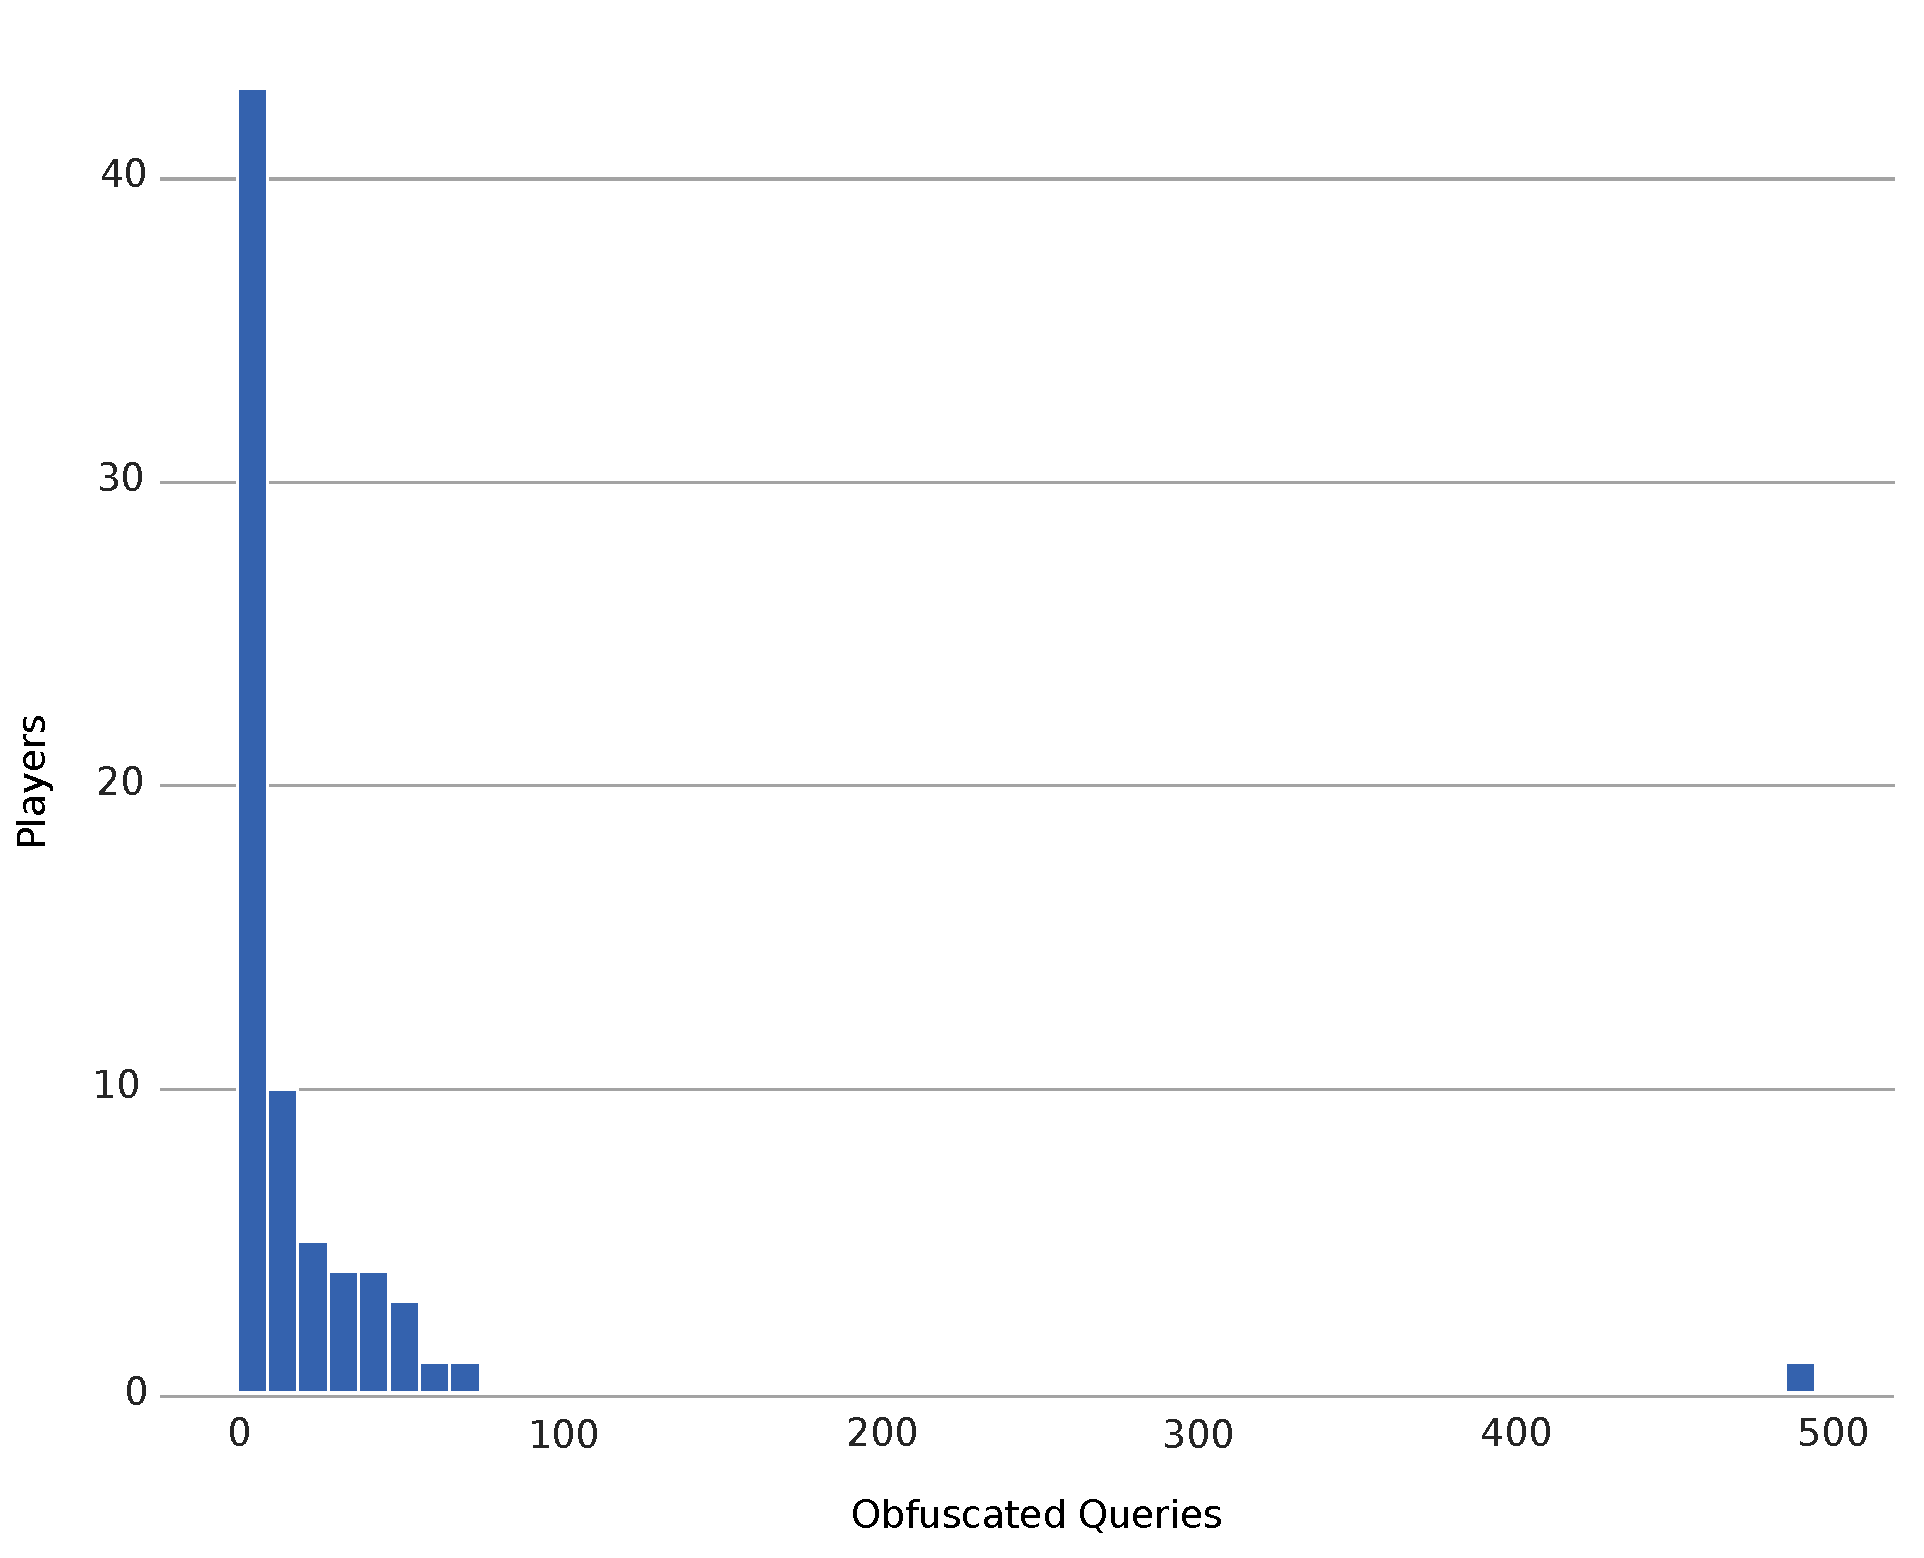
\includegraphics[width=0.7\textwidth]{graphics/evaluation/distribution_num_submitted_queries.pdf}
    \caption{Distribution of the amount of obfuscated queries among the players.}
    \label{fig:distribution:num:queries}
\end{figure}
The collected queries spread over the two levels we implemented, Squid and Chameleon, even though most players preferred the level Squid. Only 13\% of the collected queries were made in the level Chameleon, and only 18 participants decided to play this level. This can be explained, among other things, by the fact that the second level Chameleon is only unlocked after a participant successfully obfuscated five queries. Successful in this context means that the target document was retrieved. But since numerous players submitted very few queries, many did not even reach the second level.
However, it is noticeable that approximately 79\% of the queries in the level Chameleon were created without the usage of one of the provided auxiliary keywords (see Figure~\ref{fig:chameleon:intention}). This shows that the intention behind the level, to encourage the players to be more creative, was successful, even if the level itself was not very popular.\par
\begin{figure}[h]
    \centering
    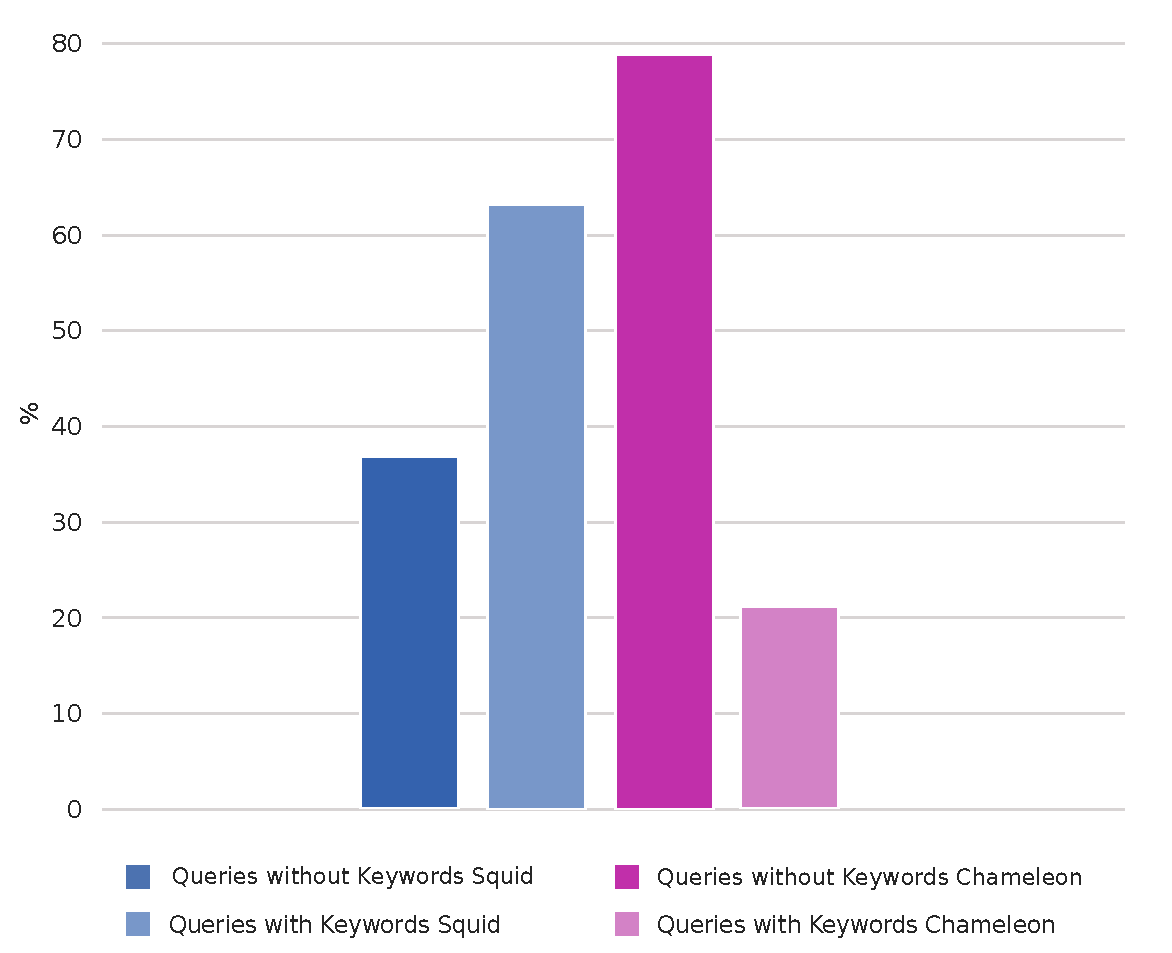
\includegraphics[width=0.6\textwidth]{graphics/evaluation/query_used_keyword_test_success_chameleon_purpose.pdf}
    \caption{The distribution of queries that were created with the help of a provided keyword.}
    \label{fig:chameleon:intention}
\end{figure}
Apart from the levels, there were also differences in the popularity of the individual categories. This can be seen from the number of obfuscated queries in each category (see Figure~\ref{fig:distribution:level:queries}). The category Knowledge was by far the most favored. If we look at the level Squid, almost all other categories are equally popular, except for Law. In the level Chameleon, the differences between the categories are not completely the same as in the other level but even here the category Knowledge was the most popular and law the most disliked. This is an interesting distribution since it shows that the number of sensitive queries in one category is not related to the number of obfuscated queries in this category. Because if this were the case then most queries would have been obfuscated in the categories Health and Personal. But these are on par with a category like politics which does not even consist of half as many queries.\par
\begin{figure}[h]
    \centering
    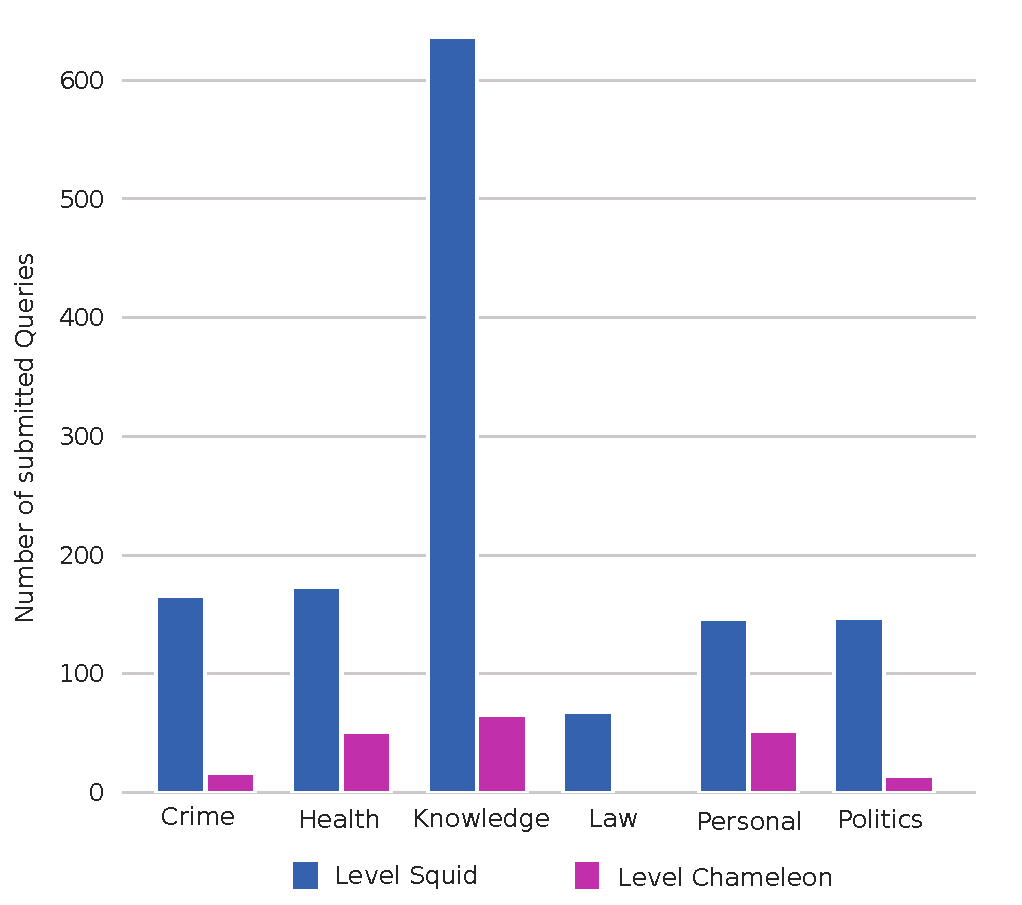
\includegraphics[width=0.6\textwidth]{graphics/evaluation/queries_per_category.pdf}
    \caption{This graph shows the number of obfuscated queries that were submitted in each category and level.}
    \label{fig:distribution:level:queries}
\end{figure}
Although there are differences in the popularity of the different queries, we can see that in each category the average length (in terms) of the created queries was longer than the original sensitive queries (see Figure~\ref{fig:distribution:length:categories}). 
\begin{figure}[h]
    \begin{minipage}[b][][b]{0.47\textwidth}
        \centering
        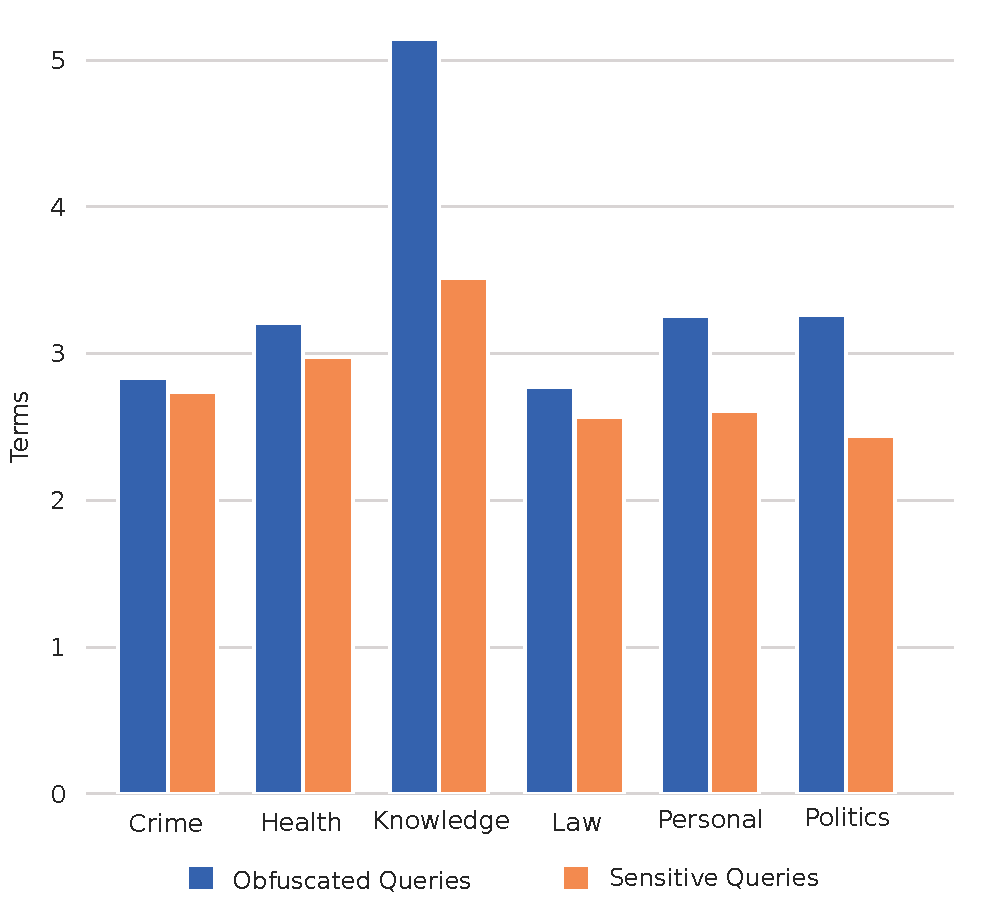
\includegraphics[width=1.0\textwidth]{graphics/evaluation/queries_length_comparison_original_categories.pdf}
                \caption{Comparison of the average length of the obfuscated queries with the sensitive queries in each category.}
    \label{fig:distribution:length:categories}
    \end{minipage}
    \hfill
    \begin{minipage}[b][][b]{0.47\textwidth}
        \centering
        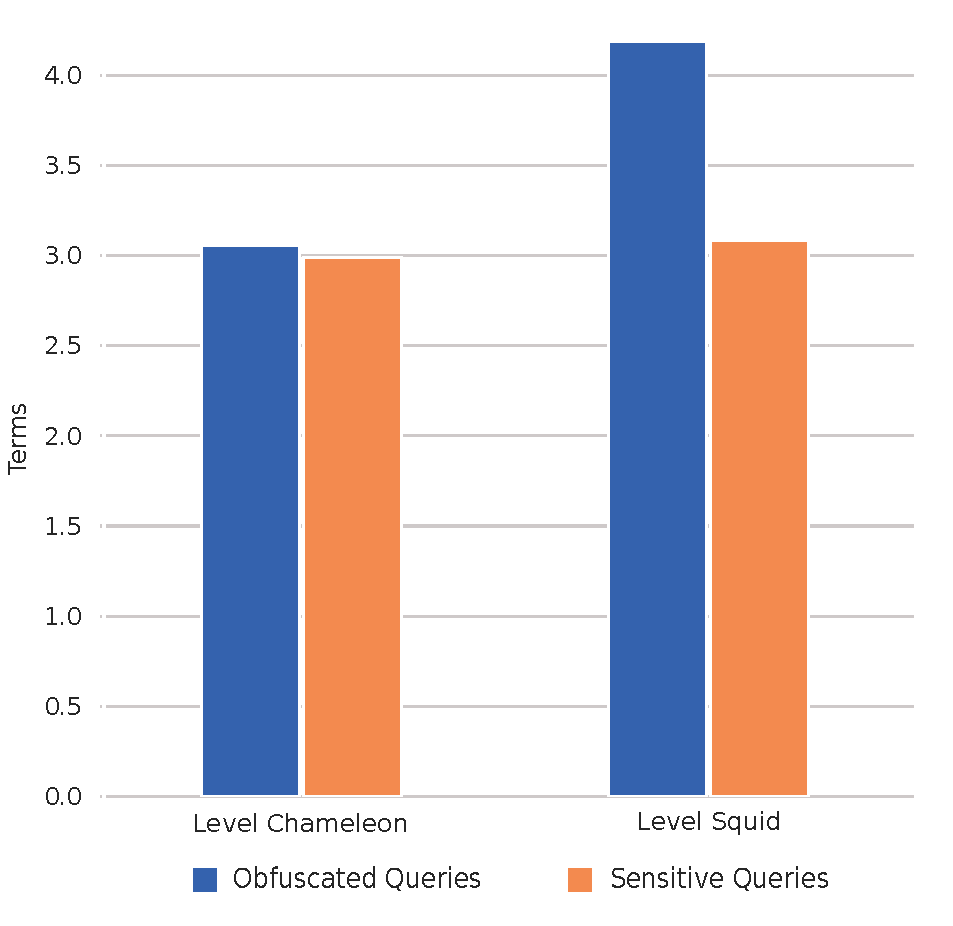
\includegraphics[width=1.0\textwidth]{graphics/evaluation/queries_length_comparison_original.pdf}
                    \caption{Comparison of the average length of the obfuscated queries with the sensitive queries in the two levels.}
        \label{fig:distribution:length:level}
    \end{minipage}
\end{figure}
The most significant difference in length can be seen in the category Knowledge. Also mentionable is the fact that the length difference between the sensitive and obfuscated queries is bigger in the level Squid than in the level Chameleon (see Figure~\ref{fig:distribution:length:level}). 
This discrepancy could be explained by the different number of submitted queries and players between the two levels. More distinct players and queries hold more potential for different approaches when it comes to obfuscating queries. Additionally, the level Squid contains the longest obfuscated query with 55 terms which also increases the average length for this level.
In general, the average length of the submitted queries is 4.04 which is in the normal range of 2-4 terms~\cite{arampatzisLength}. Figure~\ref{fig:distribution:length} shows that most submitted queries have a length of 2-4 terms but longer queries also occur. However, the length of the obfuscated queries is above the average length of the sensitive queries, which is 3.07 terms. Other sources also indicate that normal queries are on average 3.31~\cite{fu-finder} or 3.5~\cite{pictureSearch} terms long. Even though these sources show a slight deviation among themselves, their values are still lower than our value for the average length of the obfuscated queries.\par


\begin{figure}[b]
    \vspace*{-.5cm}
    \begin{minipage}[b][][b]{0.45\textwidth}
    \centering
    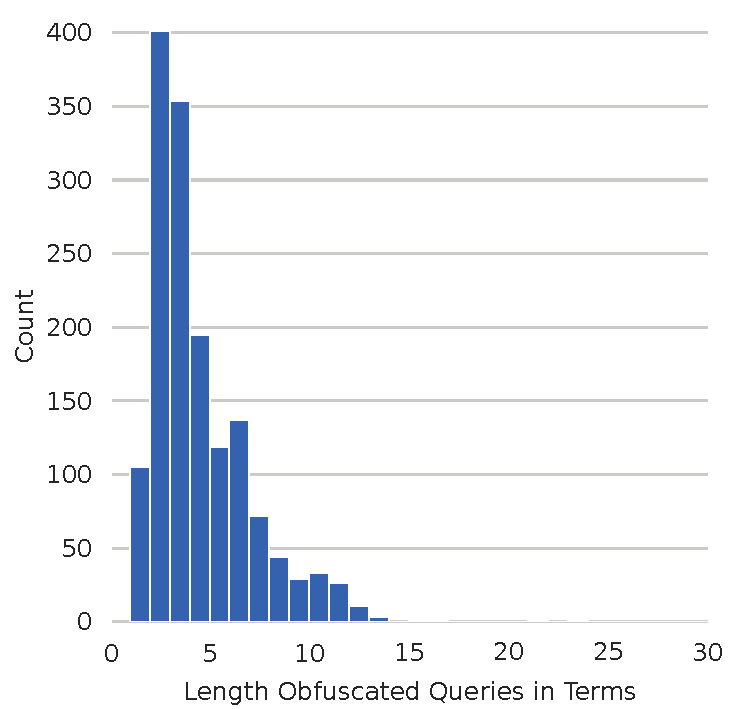
\includegraphics[width=1.0\textwidth]{graphics/evaluation/distribution_length_submitted_queries.pdf}
    \caption{The distribution of the length of the obfuscated queries.}
    \label{fig:distribution:length}
    \end{minipage}
    \hfill
    \begin{minipage}[b][][b]{0.45\textwidth}
    \centering
    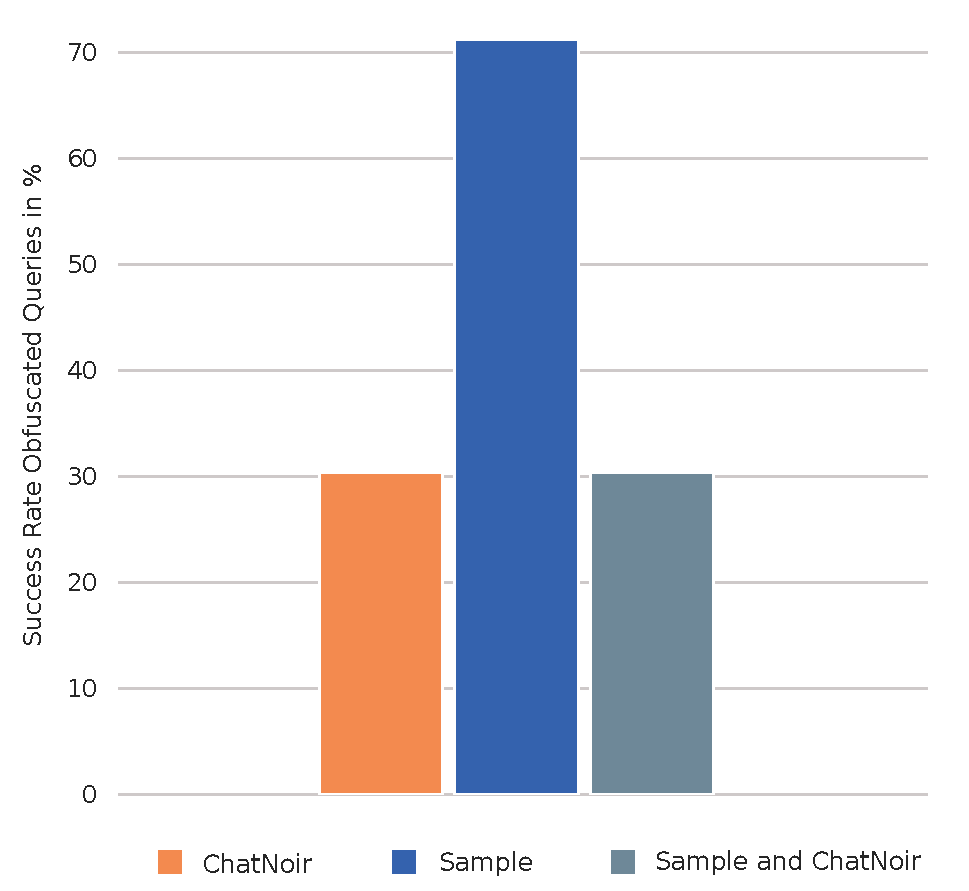
\includegraphics[width=1.0\textwidth]{graphics/evaluation/successrate_users.pdf}
    \caption{Success rate of queries in ChatNoir and our document sample.}
    \label{fig:successrate:users}
    \end{minipage}
\end{figure}
Another aspect that we investigated is the overall success rate of players. The success rate is defined as the percentage of queries that successfully retrieved the target document. As Figure~\ref{fig:successrate:users} shows, the success rate in the document sample (Index) is more than twice as high as the success rate in the ClueWeb12 (70\% compared to 30\%). We can also see that if the target document gets retrieved in ChatNoir then it also gets retrieved in our sample. Another thing we can deduce from this graph is the fact that most people were successful in their obfuscation attempts. This indicates that players did not quit the game out of frustration. 
The large difference in the success rates in ChatNoir and our sample is also reflected in the Mean Reciprocal Rank of the obfuscated queries. As we can see in Figure~\ref{fig:mrr}, the Mean Reciprocal Rank in the index is multiple times higher than the rank in ChatNoir. This trend also holds for all the query categories. Again, the most significant category is Knowledge with the largest ranking difference between ChatNoir and the document sample. Furthermore, Knowledge has the best Mean Reciprocal Rank in the sample out of all categories.
The differences in the success rate and the ranking can easily be explained by the smaller number of documents in our sample (0.6 million vs. 638.8 million).
We can directly compare the results because  our index and ChatNoir use similar retrieval models (BM25 vs. BM25F).\par


\begin{figure}[t]
    \vspace*{-.5cm}
    \begin{minipage}[b][][b]{0.45\textwidth}
    \centering
    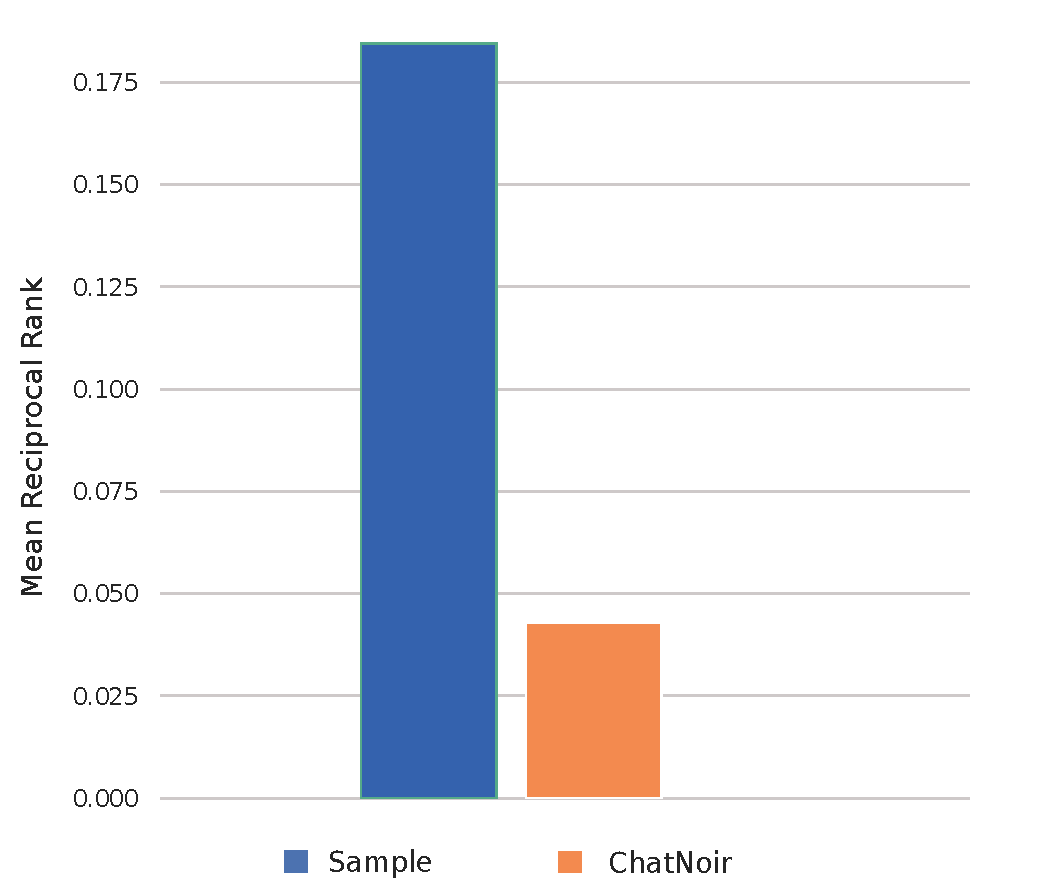
\includegraphics[width=1.0\textwidth]{graphics/evaluation/mrr_index_cw12.pdf}
    \end{minipage}
    \hfill
    \begin{minipage}[b][][b]{0.45\textwidth}
    \centering
    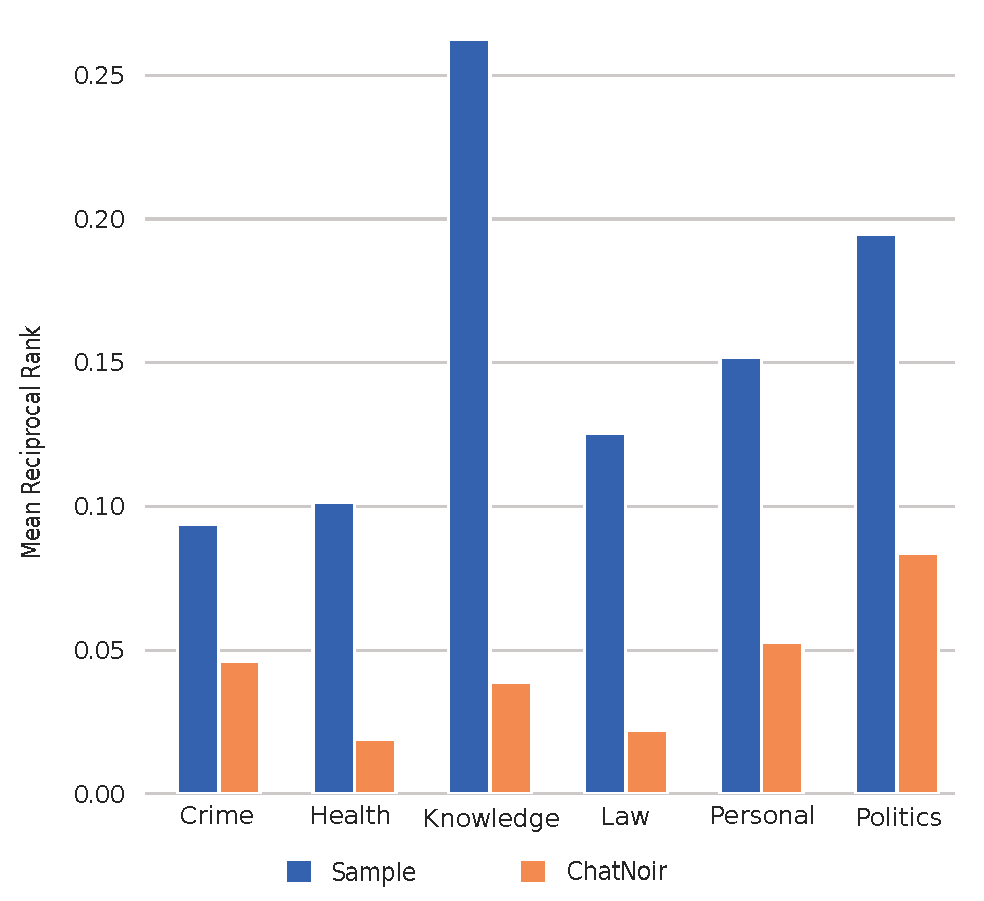
\includegraphics[width=1.0\textwidth]{graphics/evaluation/mrr_categories_both_level.pdf}
    \end{minipage}
\caption{Comparison of the Mean Reciprocal Rank for the obfuscated queries in our document sample and ChatNoir, divided into the different categories.}
    \label{fig:mrr}
\end{figure}


Through our research, we were able to identify five different query types or formulation strategies: Creative, Only Suggestions, Some Suggestions, No Suggestions, and New Word. Queries that belong to the category Creative neither contain a single word from the provided keyword list nor a word from the target document. Only Suggestions are queries that are completely made out of words from the keyword list. Queries from Some Suggestions contain at least one word from the keyword list and one additional word that is not part of the list. No Suggestions are queries that do not contain any words from the list and the last type New Word consists out of queries that have at least one term that does not come from the target document. In Figure~\ref{fig:querytypes} we can see the number of queries that belong to each query type. Note that some queries can belong to more than one type. The least used category is Creative. Although 26 players have used this strategy at least once, the proportion of queries in this category is very low. This could be due to the success rate of 0\%, which results from the BM25 ranking function. This search function needs at least one word from the target document to be able to retrieve it. We can also see this if we compare the success rate of the different categories. Figure~\ref{fig:queries:success} shows that the queries that contain at least one keyword from the list are the most successful. But the query type Only Suggestions is also not very popular. This could indicate that humans automatically try to formulate meaningful queries for them instead of simply stringing keywords together even if this would be more effective.
In the following, we will have a further look at the four query types that have a chance of retrieving the target documents.\par

\begin{table*}[t!]
    \setlength{\tabcolsep}{0.2em}
    \caption{Overview of the effectiveness of obfuscated queries in ChatNoir and the games' document sample (`Sample'). We report the Mean Reciprocal Rank (MRR), the number of documents retrieved for the original query (`Ori.'), and the number of retrieved relevant documents (`Rel.'). We show results for automatically obfuscated queries and four different types of queries submitted by players.}
    \label{table-evaluation}
    \tiny
    \begin{tabular*}{\textwidth}{@{\extracolsep{\fill}}ll@{\qquad}ccc@{\quad}cc@{\quad}cc@{\quad}cc@{\quad}cc@{}}

        \toprule

        & & & & & \multicolumn{4}{@{}c@{\quad}}{\textbf {Our Sensitive Queries}} & \multicolumn{4}{@{}c@{\quad}}{\textbf {Sensitive Web Track Queries}}\\
        
        \cmidrule(r{1em}){6-9} \cmidrule(r{.1em}){10-13}
        
        & & \multicolumn{3}{@{}c@{\quad}}{Obfuscated Queries} & \multicolumn{2}{@{}c@{\quad}}{ChatNoir} & \multicolumn{2}{@{}c@{\quad}}{Sample} & \multicolumn{2}{@{}c@{\quad}}{ChatNoir} & \multicolumn{2}{@{}c@{\quad}}{Sample}\\

        \cmidrule(r{1em}){3-5} \cmidrule(r{1em}){6-7} \cmidrule(r{1em}){8-9} \cmidrule(r{1em}){10-11} \cmidrule(r{.1em}){12-13}

        & & Count & Length & Time & MRR & Ori. & MRR & Ori. & MRR & Rel. & MRR & Rel. \\

        \midrule

        \multirow{4}{*}{\rotatebox[origin=c]{90}{\parbox[c]{4em}{\centering \textbf{Queries}}}}
        & Only Suggestions & \phantom{0}130\,/\,21\phantom{0} &  2.42 & 40.50\,s & 0.093 & 5.223 & 0.325 & 67.592 & 0.010 & 3.094 & 0.152 & 3.691\\
        
        & Some Suggestions & \phantom{0}556\,/\,125 & 4.53 & 42.45\,s & 0.046 & 4.667 & 0.258 & 85.829 & 0.013 & 3.632 & 0.038 & 3.568 \\
        
        & No Suggestions & \phantom{0}576\,/\,157 & 2.88 & 44.39\,s & 0.029 & 2.935 & 0.082 & 38.932 & 0.015 & 1.783 & 0.024 & 3.316 \\
        
        & New Word & \phantom{0}559\,/\,158 & 3.57 & 46.27\,s & 0.002 & 1.517 & 0.051 & 49.992 & 0.002 & 1.235 & 0.005 & 2.790 \\

        \midrule

        %\multirow{3}{*}{\rotatebox[origin=c]{90}{\parbox[c]{10em}{\centering \textbf{Au}}}}
        & Automatic & 1025\,/\,327 & 2.91 & --- & 0.088 & 9.229 & 0.420 & 84.264 & 0.014 & 2.872 & 0.042 & 3.743 \\
        
        \bottomrule

    \end{tabular*}
    \vspace*{-2ex}
\end{table*}

Table~\ref{table-evaluation} compares the effectiveness of the query types between each other and to queries automatically obfuscated with the approach of Arampatzis et al.~\cite{arampatzis}. Apart from the data on the different query types, the table shows an additional distinction of the queries into the sensitive queries from the Web Tracks (Sensitive Web Track Queries) and the queries from other sources in our collection (Our Sensitive Queries). For our sensitive queries, we report the Mean Reciprocal Rank (MRR) for finding the target document and the number of retrieved documents from the top-300 ranking when the original sensitive query is submitted (Ori.).
For the Web Track queries with relevance judgments, we report the MRR and the number of retrieved relevant documents (Rel.). The data indicates that the less players relied on the suggested keywords, the more time they needed to formulate their queries thus becoming less efficient (40.50 s vs. 46.27s). Overall, the time taken for the obfuscations is 40.72 seconds on average. Since we do not know how long people normally need to formulate queries, we cannot say anything about whether this is within the normal range or make any kind of comparison. But since there exist some cases in which the needed time exceeds this average value by far, there must have been some players that took their time to thoroughly inspect the provided information.\par
As expected and as we have seen before, the MRR for the index is always better than for ChatNoir which is caused by the difference in the number of documents.
Based on our collected data we can conclude that the further players deviates from the provided keywords, the less effective their query will be. This is equally true for the target web page, the number of related or relevant documents as well as the time taken to formulate an obfuscated query. If we compare the obfuscated queries of humans with automatically generated queries, then we see that players who use only terms from or list of keywords (Only Suggestions) slightly improve upon automatic obfuscation (MRR of 0.093 vs. 0.088). But for all other query types, this does not hold. On the contrary, the MRR for the automatic queries exceeds the MRR for the human-made queries. This is especially the case for the category New Word for which the obfuscations are rather useless (MRR of 0.002). With an MRR this low, no real search engine user would look at the target document, since most of them are not even interested in documents positioned worse than the tenth result~\cite{pictureSearch}. The findings of this paragraph are also confirmed by the data of the sensitive Web Track queries.
\begin{figure}[ht!]
    \vspace*{-.4cm}
    \begin{minipage}[b][][b]{0.45\textwidth}
    %\centering
    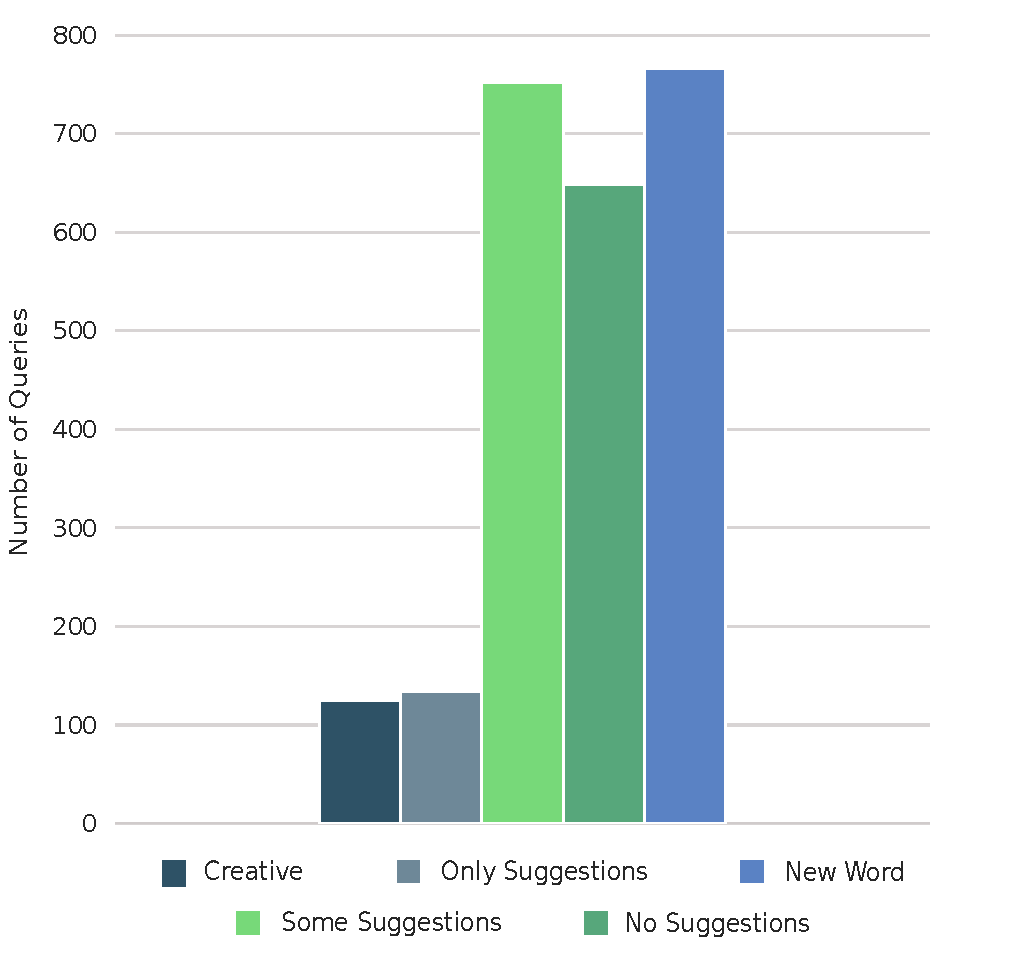
\includegraphics[width=1.0\textwidth]{graphics/evaluation/five_query_categories.pdf}
    \caption{Overview of the number of queries in each query type.}
    \label{fig:querytypes}
    \end{minipage}
    \hfill
    \begin{minipage}[b][][b]{0.45\textwidth}
    %\centering
    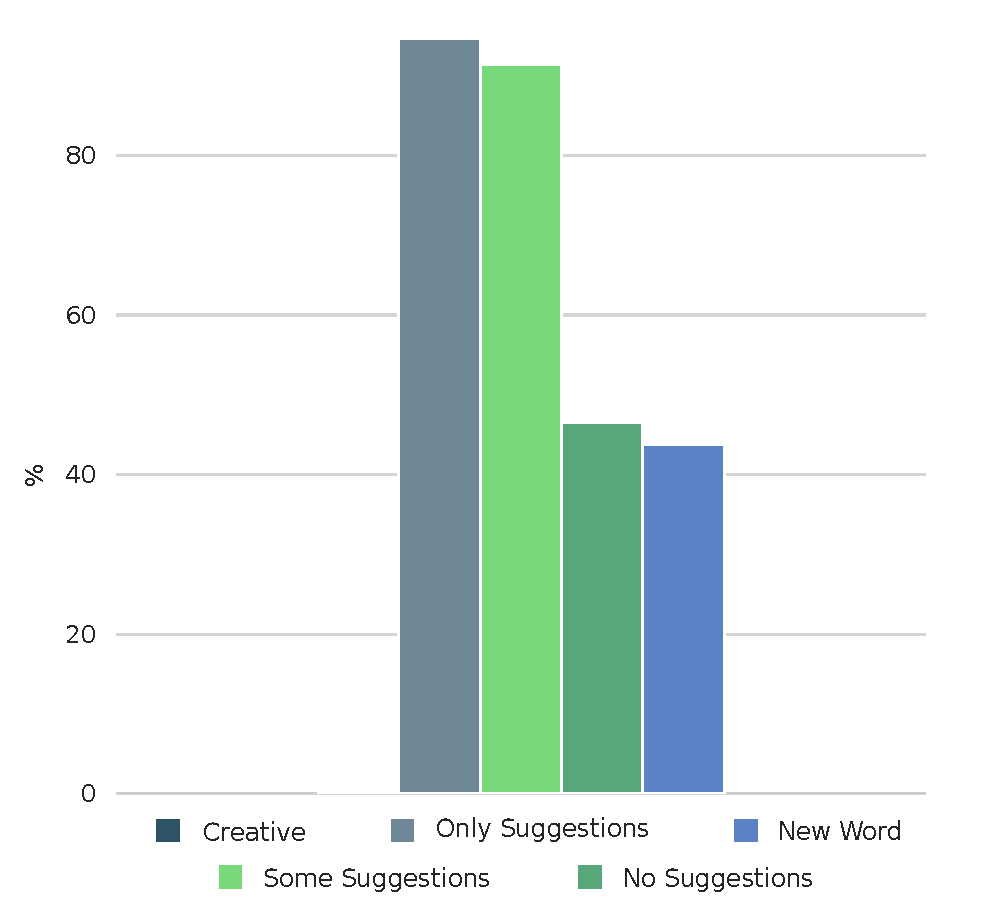
\includegraphics[width=1.0\textwidth]{graphics/evaluation/five_query_categories_success_rate.pdf}
    \caption{Overview of the success rate of players for each query type.}
    \label{fig:queries:success}
    \end{minipage}
\end{figure}



\chapter{Conclusion and Future Work}
The goal of this thesis is to research how effective humans can retrieve relevant web pages while obfuscating sensitive information needs as well as the strategies they pursued. To collect as much data as possible and to get more people interested in participating in our research, we decided to use gamification. Therefore, we developed City of Rebellion, a web game in which players must reformulate a given sensitive query without using any of the terms it consists of. To make this task easier, the game interface includes a list of auxiliary keywords and a web page relevant to the sensitive query.\par
Through the game's logs, we were able to gather data about the effectiveness and efficiency of players, and their strategies for obfuscating queries. We find that the obfuscated queries are on average slightly longer than the sensitive queries but still in the normal range of 2-4 terms. We study the effectiveness and efficiency of obfuscated queries belonging to five strategies (Creative, Only Suggestions, Some Suggestions, No Suggestions, and New Word). These types differ in their effectiveness and efficiency. We find that the efficiency as well as the effectiveness decrease the more players deviate from suggested obfuscation terms. If we compare the effectiveness of the player's queries with queries generated with the approach of Arampatzis et al.~\cite{arampatzis}, the automatically obfuscated queries are more effective in almost all cases.
Based on our research, we conclude that people would not be able to retrieve documents easily, if they would not be provided some kind of additional information, e.g. our suggested terms. Additionally, our results suggest that the effectiveness of obfuscated search queries depends on the size of the index, with higher effectiveness on small indexes and lower effectiveness on large indexes. 
And since commercial search engines like Google have indexed many more documents than ChatNoir or our sample, the effectiveness would probably decrease even further than in our findings.
This means that people have to rely on obfuscation techniques like the approach of Arampatzis et al.~\cite{arampatzis} if they want to hide their sensitive information needs.\par
In the future, we would like to collect more query obfuscations from different population groups. For this thesis, we only gathered data of people in the context of universities, especially from the computer science departments. However, this does not reflect the people who use search engines. Therefore, we make our game accessible to a broad spectrum of players and try to advertise it on suitable conferences. 
Furthermore, we want to add more retrieval algorithms to the game to research the effectiveness of different retrieval models and the effectiveness of obfuscated queries on larger indexes. We also consider to develop a mobile version for smartphones which could potentially lead to more players. Our collected data also holds the possibility for more research aspects like the choice of terms of players. The research possibilities are not limited to the aspects we investigated in this thesis.\par
In any case, we hope that this research will help to develop better search privacy algorithms and to comprehend human query obfuscations.

\printbibliography
\end{document}
